\documentclass{report}

\usepackage{pdfpages}
\usepackage{comment}
\usepackage{titlesec}
\usepackage{blindtext}
\usepackage[most]{tcolorbox}
\usepackage{graphicx}
\usepackage{float}
\usepackage{fancyvrb}
\usepackage{hyperref}
\usepackage[toc,page]{appendix}
\usepackage{ulem}
\usepackage{pgfgantt}
\graphicspath{ {./Images/} }

\usepackage[left=3cm, right=3cm]{geometry}

\makeatletter
\NewDocumentCommand{\mynote}{+O{}+m}{%
  \begingroup
  \tcbset{%
    noteshift/.store in=\mynote@shift,
    noteshift=1.5cm
  }
  \begin{tcolorbox}[nobeforeafter,
    enhanced,
    sharp corners,
    toprule=1pt,
    bottomrule=1pt,
    leftrule=0pt,
    rightrule=0pt,
    colback=yellow!20,
    #1,
    left skip=\mynote@shift,
    right skip=\mynote@shift,
    overlay={\node[right] (mynotenode) at ([xshift=-\mynote@shift]frame.west) {\textbf{Note:}} ;},
    ]
    #2
  \end{tcolorbox}
  \endgroup
  }
\makeatother

\newcommand{\req}[2]{\textbf{		#1:  }	\textit{#2}\newline\newline}

\titleformat{\chapter}[block]
  {\normalfont\huge\bfseries}{\thechapter.}{1em}{}
\titlespacing*{\chapter}{0pt}{-19pt}{0pt}

\begin{document}

\title{
Final Report \\ 
\textit{3D Video Game: Star And Salvation} }
\author{267533\\
\large Word Count: 10700}

\maketitle

\tableofcontents

\chapter{Introduction}
While the written word can gain a form of dynamism through ambiguity, applying that to an interactive and visual medium becomes challenging to do concretely. Instead, gameplay elements, such as simulation and customisation, can be used to engender a narrative in the player, giving them the space to fill in the gaps in their own minds. When done well even non impactful decisions can be imbued with a sense of weight, this feeling that everything contributes. On the other end when done poorly, all decisions can become meaningless whether they are impactful or not. What matters is the player believing they're having an impact. 

This form of narrative interaction is seen commonly in the large-scale real-time strategy genre (e.g. Stellaris \cite{stellaris}, Crusader Kings \cite{crusaderkings}, etc.) where interlocking systems tell the stories of large factions. The objective of this project is to first create a beta version of a game in this genre, then perform a round of user testing. Insights gained from that process will then be used to complete a vertical slice. Given the constraints inherently imposed by solo development across such a limited time scale, it is unlikely a fully finalized version of the game will be completed.

To allow the player to make immediate, impactful decisions at the beginnign of any given run, unlike most games in the genre, the player's power (i.e. their ability to affect the simulated environment) will be orgainzed differently to other entities. The player will start as a single powerful unit (i.e. a single ship, a single character, etc.) that has a decent amount of upfront power. During the early game, they will still need to make tactical decisions in order to survive but importantly they should already be able to have an effect on the game's world with a large amount of upfront ability to effect change. Alongside this, the player will be immediately presented with customization options for their entity, allowing them to customize their faction's emblem, leading them into a roleplaying headspace.

To ensure that the player's actions result in dynamic outcomes, the faction simulation will also need to be suitably complex. As such, this project takes a code-agnostic, data driven approach. This involves keeping faction data separate from any given simulation element, as opposed to a typical object-oriented approach, which would intertwine them. This allows simulation modules to be designed and implemented in a flexible manner, as well as allowing extra simulation elements to be added easily as an extension goal.

Additionally the player will be able to grow in strength throughout a run, affecting more and more of the game's world as time goes on. This can be done through statistic increases but also more dynamic and interesting item purchases. Power upgrades should always be a reward for interacting with the game's world, incentivising investment in the Simulated environment.
\newline
\newline
This report consists of several sections, the first of which is "Professional Considerations", where the BCS Code of Conduct is broken down by section. An ethical review is also included, discussing this project's plan for user testing and acquiring consent for personal data collection in detail. Next is "Requirements Analysis", which outlines the objectives of the project in distinct steps alongside expanding on the explanation of the problem space and my solutions. This includes background research on games in the genre and proposed solutions to game design issues found within, alongside a brief section on "Art Design". That subsection details some techniques used to render the large solar system as an example of some of the work done on the visual side of the game.
Next is the "Project Plan", consisting of a breakdown of the work required to complete the project into distinct phases, illustrated using a Gantt chart alongside written explanations. Then there is an "Interim Log" detailing the steps of the Project Plan completed as of the submission of this Interim Report and meetings with this project's supervisor. Finally, there are the refrences and appendices.

\chapter{Professional Considerations}

\section{BCS Code of Conduct}

The BCS Code of Conduct \cite{bcs} is composed of four key principles, the relevant sections from each have been discussed below.
\newline
\newline
\begin{raggedright}
{\Large \underline{Principle 1: You make IT for everyone}}
\newline
\newline
\textbf{1.1 Have due regard for public health, privacy, security and wellbeing of others and the environment}
\newline
\newline
\textit{Given the sci-fi nature of the project, visuals are likely to be flashy and potentially dangerous for people with epilepsy. An appropriate warning should be displayed when the game is booted. If leaderboards are added, in line with Extension Requirement E2, some player data will be stored, this will simply include game statistics and no non-public personal information. The game's potential age rating (in line with industry standards used by parents to assess what games their children should play (e.g. PEGI)) is discussed in 2.4 below.}
\newline
\newline
\textbf{1.2 Have due regard for the legitimate rights of third parties}
\newline
\newline
\textit{This project uses some third party code, namely MonitorBreak's Additions library for Unity. This is licensed under a modified MIT license\cite{additionsLicense} and all obligations outlined have been met. It should also be noted that I wrote this code but it simply belongs to a seperate entity.
If any additional third party libraries or assets are used in the future they will also be properly attributed.}
\newline
\newline
\textbf{1.3 Conduct your professional activities without discrimination on the grounds of sex, sexual orientation, marital status, nationality, colour, race, ethnic origin, religion, age or disability, or of any other condition or requirement}
\newline
\newline
\textit{Populations in the game are abstracted, represented as a series of numbers, user testing however, is relevant to this section. The project will not discriminate when deciding which users to use as a sample instead trying to get an accurate representation of the intended users.}
\newline
\newline
\textbf{1.4 Promote equal access to the benefits of IT and seek to promote the inclusion of all sectors in society wherever opportunities arise}
\newline
\newline
\textit{This game is intended to be released for free and the simulation design will be made fully open source some time after submission. These are both done to hopefully promote more games like this being created.}
\newline
\newline
{\Large \underline{Principle 2: Show what you know, learn what you don't}}
\newline
\newline
\textbf{2.4 Ensure that you have the knowledge and understanding of legislation and that you comply with such legislation, in carrying out your professional responsibilities}
\newline
\newline
\textit{The most relevant pieces of legislation center around the game's suitability for given age brackets. This project does not intend for a physical release (even upon completion of all Extension Requirements) so upon the game's completion only the IARC (International Age Rating Coalition) questionnaire will need to be completed. The questionnaire will give an age rating inline with all participating rating boards. This rating is expected to be in the 7-12 range, given the lack of direct visible violence but the presence of war in an abstract format.}
\newline
\newline
\textbf{2.5 Respect and value alternative viewpoints and seek, accept and offer honest criticisms of work}
\newline
\newline
\textit{All feedback gained from user testing will be treated with equal respect and this project will seek to make no omission when presenting it in the final report. To gain more feedback, additional rounds of user testing are considered a high priority extension objective.}
\newline
\newline
\textbf{2.6 Avoid injuring others, their property, reputation, or employment by false or malicious or negligent action or inaction}
\newline
\newline
\textit{As mentioned in the response to 1.1, steps will be taken to prevent causing issues for people with epilepsy. Additionally care will also be taken during the creation of systems that save to disk (game save system, screenshot system, etc.). This is to prevent potential loss of personal data due to an erroneous disk write operation.}
\newline
\newline
\textbf{2.7 Reject and will not make any offer of bribery or unethical inducement}
\newline
\newline
\textit{During user testing feedback will be gathered anonymously, with no incentive for a better or worse response.}
\newline
\newline
\underline{For this project, Principle 3 and Principle 4 contain no relevant sections.}
\end{raggedright}

\section{Ethical Review}

This project requires user testing, the nature of the testing is discussed in detail in Requirements Analysis section 3.2.
Due to the use of human participants, an ethical review utilizing Sussex's standard Ethical Compliance Form needs to be performed.

A signed copy of this form is included as an appendix.
\begin{raggedright}
\newline
\newline
\textbf{1. Participants were not exposed to any risks greater than those
encountered in their normal working life.}
\newline
\newline
The game includes no visuals, audio or content that pose a significant risk to participants. Their involvement will include only playing the game and answering questions.
\newline
\newline
\textbf{2. The study materials were paper-based, or comprised software
running on standard hardware.}
\newline
\newline
The game will run on a standard Windows machine, Google Forms will be used to receive anonymous answers and will be accessed using the same machine.
\newline
\newline
\textbf{3. All participants explicitly stated that they agreed to take part,
and that their data could be used in the project.}
\newline
\newline
It will be made clear to all participants the nature of the project, all participants will be required to sign a standard consent form for data usage. It will be made clear that they can leave at any time should they no longer feel they want to take part.
\newline
\newline
\textbf{4. No incentives were offered to the participants.}
\newline
\newline
No participants will be offered any incentive for participating, they will all be volunteers attending the university. No incentive will be given to give a particular type (positive or negative) of feedback.
\newline
\newline
\textbf{5. No information about the evaluation or materials was intentionally withheld
from the participants}
\newline
\newline
Participants will be told upfront the full scope and nature of the project.
\newline
\newline
\textbf{6. No participant was under the age of 18}
\newline
\newline
All participants will have their ages verified prior to their participation.
\newline
\newline
\textbf{7. No participant had a disability or impairment that may limit their understanding
or communication.}
\newline
\newline
All participants will be able-bodied university students, that they are in an appropriate state of health will be verified prior to user testing.
\newline
\newline
\textbf{8. Neither I nor my supervisor is in a position of authority or influence over any of
the participants.}
\newline
\newline
All participants will be my university peers and none will share my supervisor if they are also doing their final year project. Their feedback will also be kept separate from their identity to ensure they cannot be linked to particular criticism.
\newline
\newline
\textbf{9. All participants were informed that they could withdraw at any time.}
\newline
\newline
It will be made clear to all participants, both at the beginning and at various stages throughout the process, they are allowed to withdraw (for any reason) at any time.
\newline
\newline
\textbf{10. All participants have been informed of my contact details, and the contact details
of my supervisor.}
\newline
\newline
This information will be provided on a separate piece of paper, alongside a basic written breakdown of the project.
\newline
\newline
\textbf{11. The evaluation was discussed with all of the participants at the end of the
session, and all participants had the opportunity to ask questions.}
\newline
\newline
Participants will be allowed to ask questions at any point during the process. Appropriate time will be allocated at the end of the user testing session to allow for additional questions and a discussion on the evaluation.
\newline
\newline
\textbf{12. All the data collected from the participants is stored securely, and in an
anonymous form.}
\newline
\newline
All responses will be secured behind access to my password and 2FA protected google account before being moved to my password protected PC. Any identifiable information will be redacted.
\end{raggedright}

\chapter{Requirements Analysis}

This project aims to produce a player-story driven RTS (Real Time Strategy). in the form of a vertical slice (a version of a game that lacks some features but still showcases what the final product will look like). The game's world will need to be deeply simulated, comprising a large amount of the technical challenge of the project.

\section{Framework Choice}
This project uses Unity \cite{unity} instead of a custom engine, the primary reason for this choice is my familiarity with it's workflow. I've previously created a full game using Unity (including shipping it to Steam \cite{steam}) and I greatly enjoy its flexibility. Unity makes it easy to extend the editor through creating additional context menu items and entirely new editor tools. 
The C\# (which is Unity's primary coding language) ecosystem is also very broad, with a colossal number of resources to pull from. 

I additionally chose not to use this project as an opportunity to learn a new engine as no other contemporary engines seemed fit to purpose. Unreal \cite{unreal} includes many systems that are superfluous for this project (e.g. Blueprints, Nanite, etc.) and I'm also unfamiliar with C++ to an extent where large practical issues could arise (such as poor design planning, language specific pitfalls, etc.). Godot \cite{godot} was initially a contender for my engine of choice (I also have some minor previous experience with it), however, I quickly found tension between myself, and it's scripting language of choice GDScript. The primary issue that arose during testing is that I wanted engines to work similarly to Unity when they had clear differing approaches to design (e.g., Godot's node based workflow).

\section{User Testing}
To assist with the development process, at least one round of in-person user testing should occur. This would involve allowing a number of potential users (ideally 5+) to play the game for a period of time before asking them a sequence of questions.

The sample of players should be made up of both people familiar with the RTS genre and those that are not, ideally spread evenly across that range. Ideally two primary testing rounds should occur, one once an inital beta version of the game is produced and one afterward, utilizing the vertical slice. The beta version can differ from the vertical slice dramatically in terms of completeness but should still be functional.
The vertical slice testing (and any additional testing) is helpful but should be considered an extension objective given the time constraints.

\pagebreak
\section{Background Research, Design Problems and Solutions}

\subsection{Game 1: Stellaris}

Stellaris (2016) \cite{stellaris} is a large scale space-based strategy game, taking place across a substantially sized galaxy. It involves managing an interstellar faction, taking them from their first ships to combating a galaxy wide threat. 

The game puts a heavy emphasis on role-play right from the beginning of a run. Immediately upon selecting "New Game" you are presented with the screen pictured in Figure 3.1.

\begin{figure}[h]
    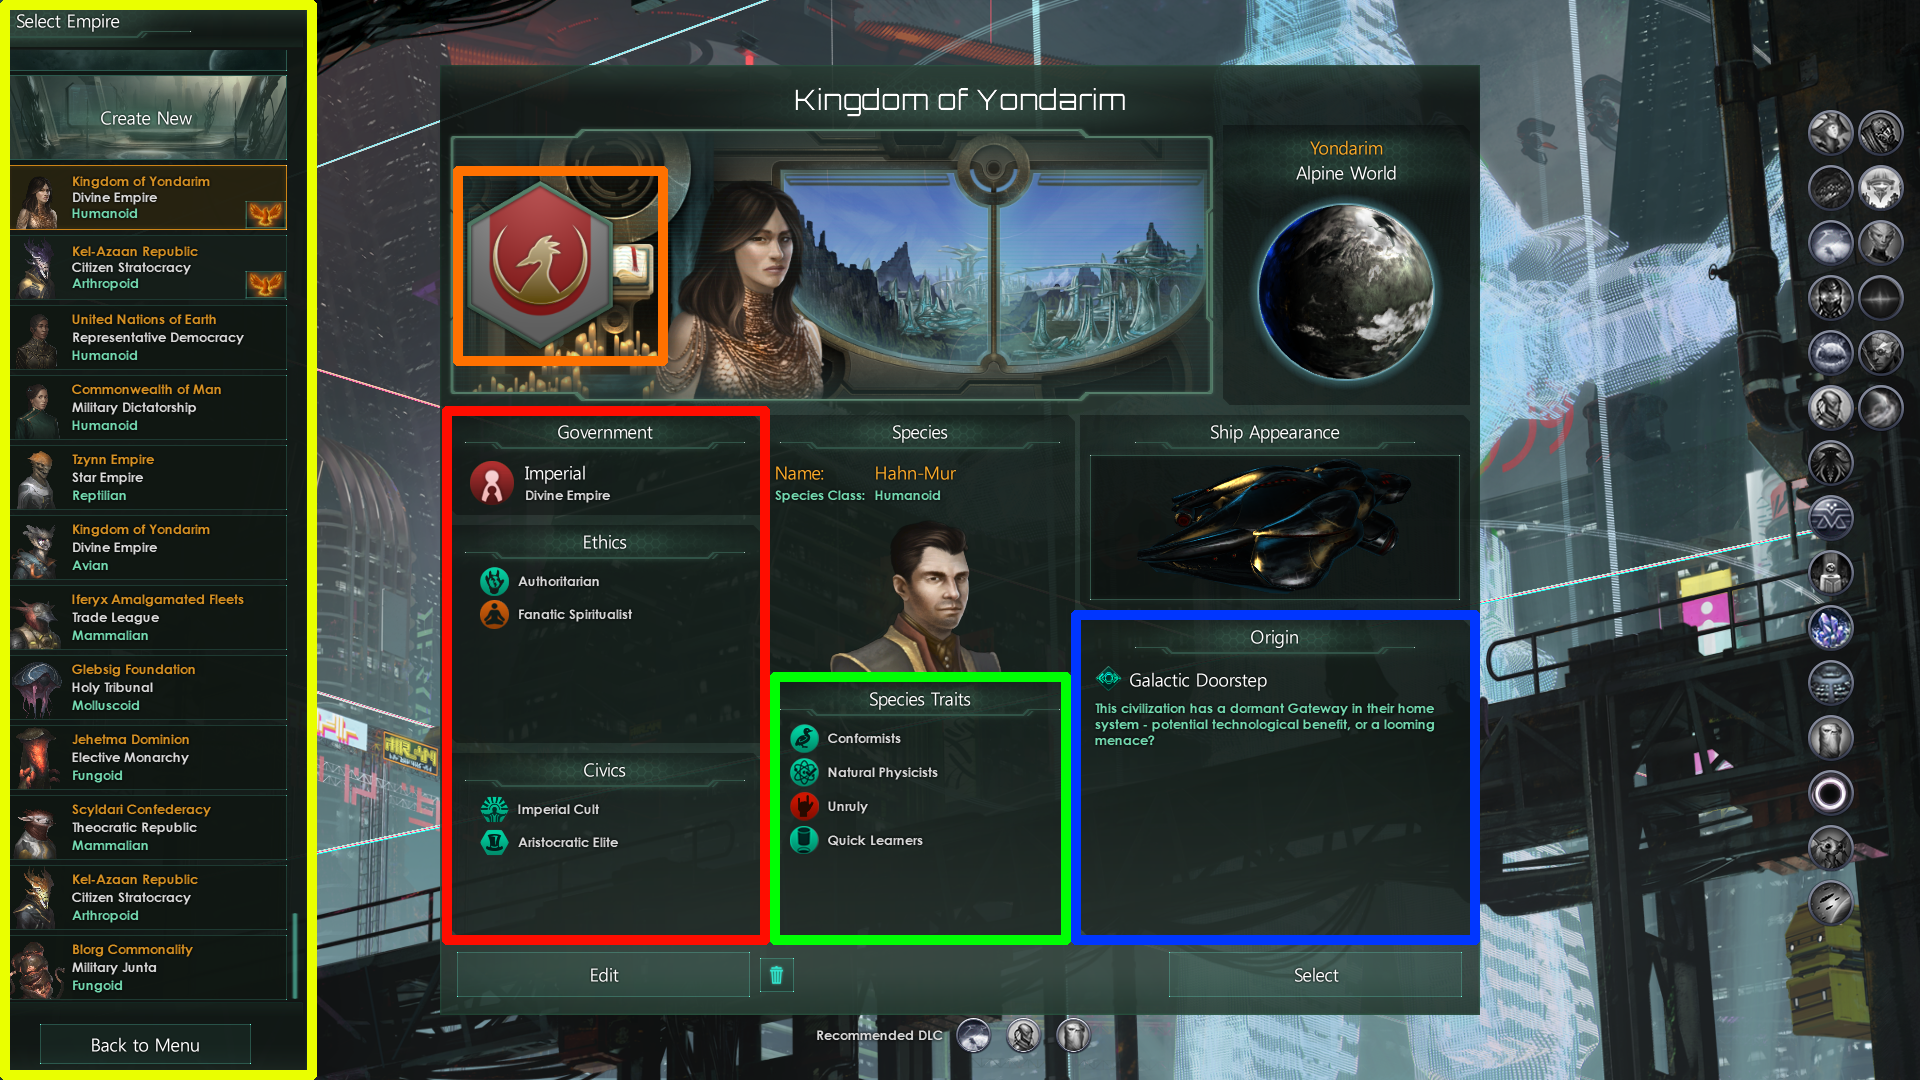
\includegraphics[width=\textwidth]{stellaris_faction_creation.png}
    \caption{Stellaris Faction Creation Screen}
\end{figure}

The left side of the screen showcases a list of premade factions (highlighted in yellow) that the player can pick from then customize, these can act as a  jumping off point for player ideas. There is additionally an option to create an entirely unique faction at the very top. 
Positioned directly in the center of the screen is the information on the currently selected faction, including; their governmental practices (highlighted in red), their species traits (highlighted in green), their species origin (highlighted in blue) and their faction's flag (highlighted in orange). All these elements (alongside others) create a distinct feeling for this particular faction and, more importantly, they have gameplay ramifications. Within a minute of starting the game proper the faction shown in Figure 3.1. (an Imperial Divine Empire) was notified it had received a new heir, a special type of unit that acted (in this case) as a scientific advisor.

This focus on role-play is reflected in the reviews for the game, many are simply retellings of their own faction's story. An example of this is pictured in Figure 3.2.

\begin{figure}[H]
    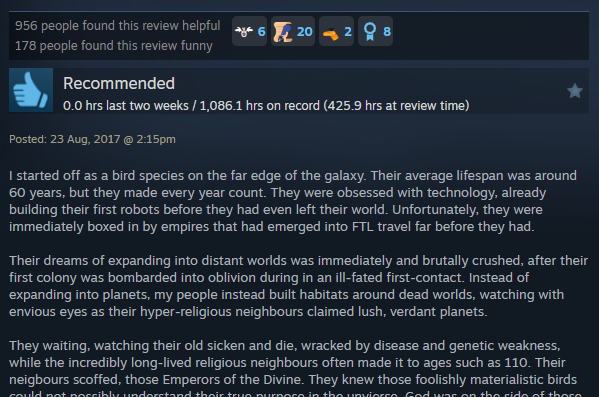
\includegraphics[width=\textwidth]{stellaris_positive_review.png}
    \caption{A retelling of a Stellaris game, (full review is 650+ words long)}
\end{figure}

Other systems also assist this storytelling, in particular the Galactic Crises. These are large, late game events that typically have ramifications for the whole galaxy and act as a definitive final boss for a play through. Interestingly, there are also specific cases where a player or AI can become the crisis, another avenue for potential role-play. The player's relationship to other factions can be vitally important during these scenarios, meaning earlier (possible role-play based) decisions can have a major impact.

Space combat is another important part of Stellaris but is more used as a tool to express role-play decisions than a system that encourages role-play itself. The functional act of combat instead enhances the grand strategy  side of the game, engagements are often won by decisions made before the battle starts. For example, the ships used by an endgame crisis, "Extradimensional Invaders", largely rely on shields as a defensive measure for their ships. This means that kinetic weapons are particular effective \cite{stellarisBattleDecision}, outfitting ships with these weapons is a decision made when they are created. When actually fighting, fleets of ships will "auto-battle" each other, with no input required by the player. While this project does focus more on a singular powerful entity, it will take a similar pre-planning approach to combat. This is in part due to the time constraints, as time spent making combat rewarding to execute takes time away from the simulation side (and main goal) of the project.
\newline
\newline
While Stellaris succeeds in many areas and is arguably (with its balance of strategy and role-play) the closest real example of this project's goal, it has a few outstanding flaws. The game has a large amount of upfront complexity, the main Stellaris wiki's Beginner Guide \cite{stellarisBeginner} is roughly 17000 words long, split into 20+ sections and subsections. Figure 3. showcases the first screen players will see outside of the faction creation menu. It hosts a suite of information, shown to the player all at once. This includes (but is not limited too); eight types of basic resources, several more advanced resources (including fleet and starbase capacity), a list of all controlled entities (planets, fleets, construction and science ships and shipyards), the current date, many links to other UI windows (including Government Control, a larger galaxy map, Species Control, Technology and Research Management) and buttons for switching map mode (it should be made clear those buttons do nothing on this screen but are still present).

\begin{figure}[H]
    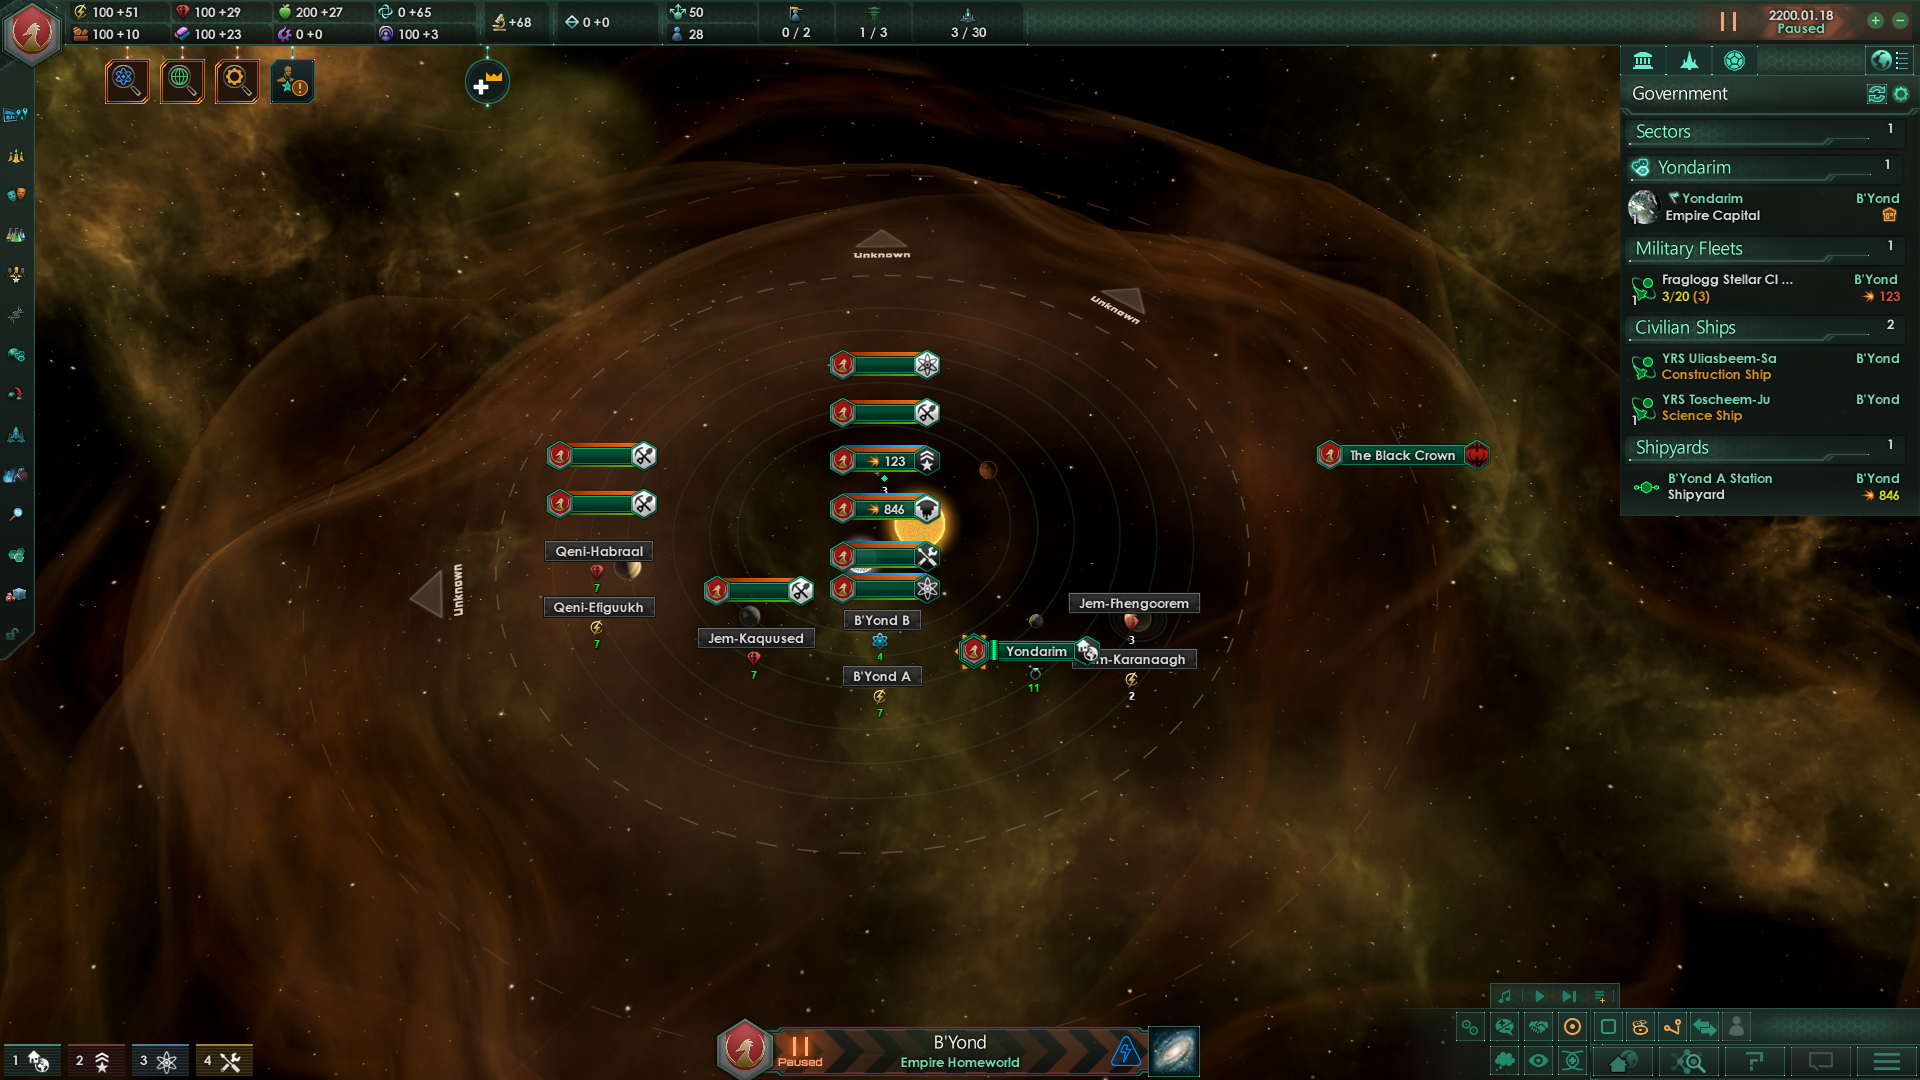
\includegraphics[width=\textwidth]{stellaris_main_screen.png}
    \caption{Stellaris Solar System View Screen}
\end{figure}

However, this complexity is an important, and arguably defining, part of the genre \cite{rtsUncertainty}. The principal issue here is how it is introduced to the player. Given this project's intention to, in part, target a wider audience, this issue is quite important. The intended solution is to introduce player elements gradually, in the context of the larger narrative brace of the game this can be expressed as the player's controlled entity turning back on after many years inactive. To enhance replayability players could be allowed to start already in a fully active state rather than repeating the tutorial each time.

Stellaris also suffers from performance issues, particularly in the late game \cite{stellarisPerformanceReview1} \cite{stellarisPerformanceReview2}. Given the relative scales of this project and Stellaris this is a less relevant issue, performance goals are discussed further in a later subsection "Performance and Stability".
\newline
\newline
One major difference between this project's game and Stellaris is that unlike a typical RTS, there will be a larger focus on the world reacting directly to the player as a singular powerful entity and less on long term historical stratergy. While the game will be in part targeted at long time RTS players, this change in power balance (alongside a shift into more role-play focused elements) is designed to allow a wider audience to engage with a typically complex genre. 

\subsection{Game 2: Disco Elysium}

This project's role-play centric aims require it to take additional inspiration from outside the RTS genre. Disco Elysium (2019) \cite{discoelysium} is a detective RPG, famous for its engaging writing. It has many systems that incentivize  role-play such as its "Thought Cabinet" system, pictured below.

\begin{figure}[H]
    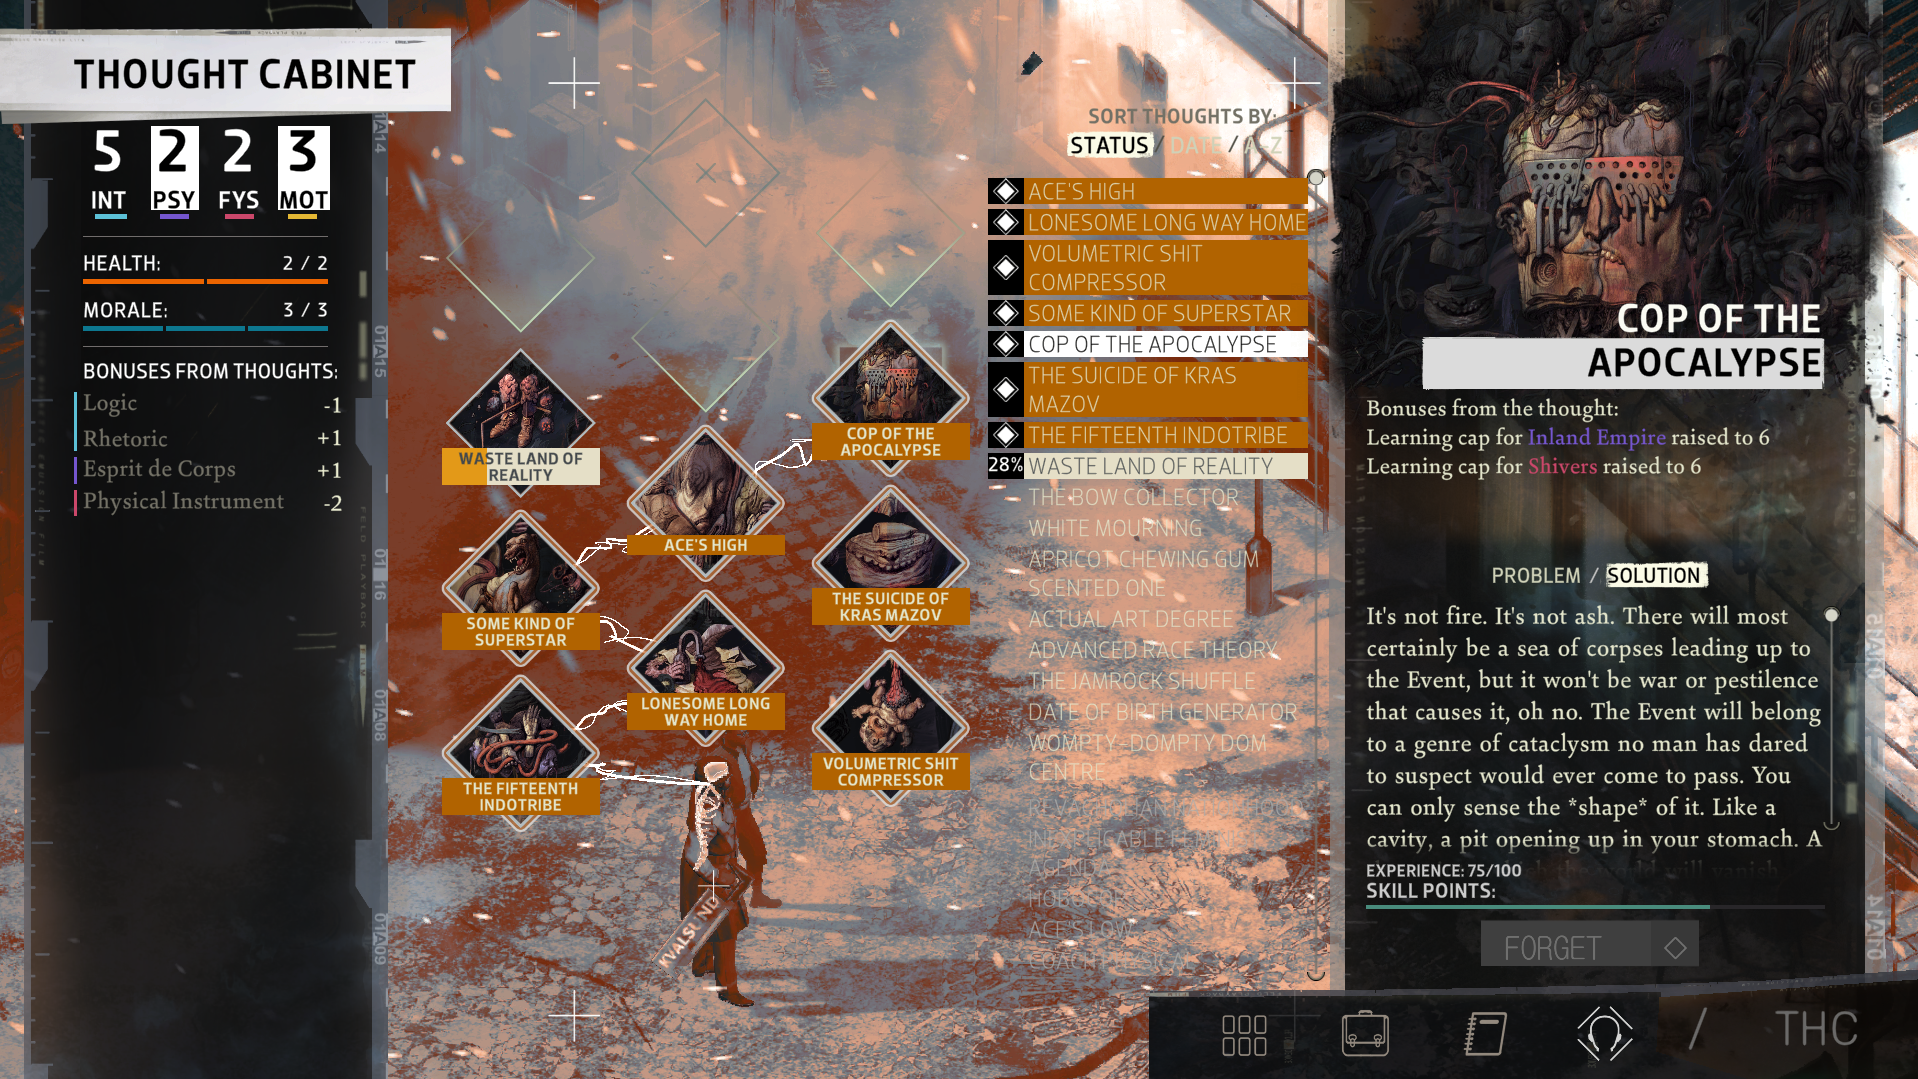
\includegraphics[width=\textwidth]{disco_elysium_thoughts_screen.png}
    \caption{Disco Elysium Thoughts Screen}
\end{figure}

"Thoughts" are discovered naturally on your adventure throughout Elysium's world, after being found they can then be slotted into an open position in the cabinet before taking some time to be "internalized". This system mirrors Stellaris's governmental polices, providing an avenue for role-play but grounding it in a more understandable mechanical benefit/cost. In the case of Disco Elysium, you use a skill point (that could be used on the game's more traditional statistics based leveling system) to unlock more slots in your cabinet. This allows players to make the active choice to engage more with role-play, potentially trading off a traditional power increase.

Disco Elysium's approach to role-play has some pain points, in particular the various bottleneck checks. The primary example is an "Authority" check during a pivotal conversation with Titus Hardie. This check (involving summing the result of two dice and your Authority value to try and meet a threshold) is necessary to move the story forward, with a low enough investment in Authority (a seemingly optional statistic up until this point), the chance to pass it can be as low as 3\%. In the context of a game trying to tell a specific story, with a character that values authority as much as Titus, this (despite the potential player frustration) works quite well, however, in this project, centered on player driven narrative, it would not. This project should seek to ensure these bottlenecks only appear in a foreseeable manner. For example, it makes sense that a faction's military will be tested if it goes to war, hence, a declaration of war should follow logically from previous choices so a player can prepare appropriately.

\section{Art Design}

Visuals are an important part of game development but they are not the focus of this report. This section will focus on the system used for large scale rendering (used for celestial bodies) as an example of some of the work done on that side of the game. 

\begin{figure}[H]
	\centering
    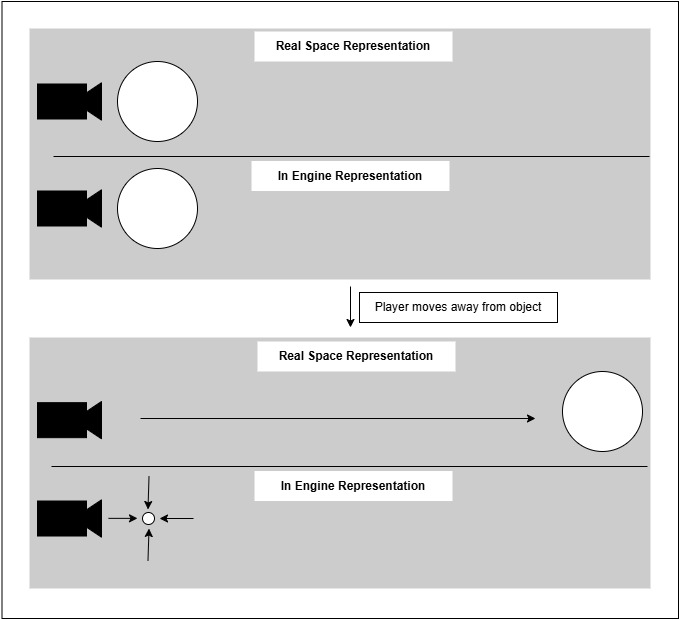
\includegraphics[width=.9\textwidth]{celestialbodiesSystemDiagram.jpg}
    \caption{1D Diagram showcasing how the celestial bodies rendering system functions.}
\end{figure}

The principal issue is Unity's use of Floats to represent positions, an effort to increase performance for the vast majority of games at the cost of precision. Given the large scale of this project's world, extra precision is key for accurate representation. 

This system takes advantage of the fact that something moving further away and something shrinking (with no point of reference) are indistinguishable. We calculate how large something should look from the player's perspective, utilizing the higher precision Double type to accurately represent the object's "real" position, before applying the reciprocal result to the object's in engine scale. This means that only the object's scale changes when the player moves and its in engine position stays close to the camera. This is showcased in the diagram above in one dimension. The principal problem is solved here because a general modifier can be applied to the final output scale, shrinking it into a range that floats can accurately represent.

 To complete the illusion all celestial objects are rendered using a separate camera and applied between the skybox and the rest of the rendered objects. This means celestial objects always appear behind (and consequently larger) than everything else.

\section{Performance and Stability}

Crashes and bugs should be kept to an ideal minimum. While the time constraints imposed don't allow the thoroughness typical of a standard project, ample time can still be allocated to unit testing and the like. The aforementioned rounds of user testing can also assist with this issue.

Alongside functioning as intended, the final version of the project should also run at a consistent and reasonable frame rate (60 frames per second) on low to medium range hardware. Given the relatively low intended visual complexity of the game, this objective is still important but easier to reach than others. Various different pieces of hardware are available for testing, with varying hardware capabilities in each.

\chapter{Formalized Requirements}
Below are the requirements discussed in the above sections formalized into a list;
\newline
\newline
\req{R1}{Existing games in the genre should be researched, their gameplay focus points, style and design problems should be identified.}
\req{R2}{User testing should be conducted with 5+ potential players, post-game interview questions should be shaped based on insights gained from completion of R1.}
\req{R3}{At least two versions of the game should be created. An initial beta version for user testing and a final vertical slice.}
\req{R4}{The game should run at at least 60 FPS on low to medium range hardware.}
\req{R5}{The game world should be suitably simulated, recognizable as realistic relationships between factions.}
\req{R6}{The player should be able to make early impactful roleplay decisions.}
\req{R7}{The game should have sound effects that fit the theming.}
\req{R8}{The player should be able to fly about their local environment.}
\req{R9}{The player should be able to travel to locations around the game world.}
\req{R11}{The player should be able to interact with their environment using defined interactions.}
\req{R12}{The player should be able to purchase and utilize items.}
\req{R13}{The player should be able to improve their statistics, examples include max health and attack power.}
\req{R14}{The game should be functionally stable, crashes should occur very infrequently.}
\req{R15}{The game should have UI that accurately describes statistics about the player's faction.}
\req{R16}{The game should have UI that accurately describes known statistics about NPC factions.}
\req{R17}{The player should be able to grow and modify their faction over time, this includes increasing military strength, increasing population and adding unique features to their faction.}
\req{R18}{The player's faction's power should be concentrated to a singular entity (e.g, one building, one ship, etc.)}
\req{R19}{The player should be able to engage in relationships, both diplomatic and hostile, with other factions.}
\req{R20}{The player's actions should be able to have a long term effect on the state of the simulation (e.g, removal of other factions, removal of settelments, etc.).}
\req{R21}{The player's singular entity should be able to engage in combat with other entites.}
\req{R22}{The player should be able to win the game in some manner but the choice to take the win should be optional. The player should be able to keep playing if they wish.}

\section{Extension Requirements}

If time allows, there are some additional requirements that would ideally be met;
\newline
\newline
\req{E1}{Additional simulation elements. For example, if the current version of the simulation models a planet's resources as a static value, a new simulation routine could decrease that value over time based on population and industrial activity.}
\req{E2}{Online functionality. This would likely take the form of online leaderboards, showcasing statistics such as "Time Survived", "Enemies Killed", "Highest Bounty", etc.}
\req{E3}{More advanced combat functionality, taking the form of additional actions on top of the existing auto battle system. }
\req{E4}{Music. While many royalty-free options exist, unique music would help set the mood properly for players.}
\req{E5}{Releasing the game on Steam. Generally speaking this is a capstone objective and would signal the end of the code side of the project. }

\chapter{Design}

\begin{comment}

Want to talk about the general modular approach to design, alongisde maybe some case studies.
Hopefully demonstrating the ways in which the simulation can naturally create gameplay patterns
	Two major ones that come to mind are: "Attacking Settlements" and "Mineral Deposits"
Also want to talk about progression 
The choice to follow a "Define as Needed" style codebase with lots of inheritance and assumed implementations.
The non frame rate tick design of the simulation
How the player interacts with the world (interactions)

\end{comment}

\section{Simulation}

\begin{comment}

Talk about the Simulation design not it's relevance to gameplay (yet)

\end{comment}

The foundation of this project is the \textbf{Simulation}, it is essential that it functions correctly and is suitably complex. It additionally needs to be flexible, the ability to swap components in and out is essential, especially in an iterative, artistic process like game development. To help fufill these requirements, core actors in the Simulation (the things being simulated, referred to as \textbf{Entities}) are composed of individual modules of data. Simulation code then runs on the data modules directly instead of the parent Entity. This \textbf{data-driven} approach has two key advantages.

\begin{enumerate}

	\item Adding functionality to an Entity is as simple as giving it an additional data module. This is typically, though not always, one line of code. Consequently, adding new Entites is also simple.

	\item Simulation systems can be self contained, acting only on the data they need to. They don't need to consider the specifics of each type of Entity that wants that functionality. This allows systems to be added quickly, without creating future considerations.

\end{enumerate}

However, a Simulation made up of fully independent data parts, could lead to a lack of interesting and divergent interaction. Consequently, this Simulation includes the ability for Simulation code to check if the owner of a data module contains another specific data module so code can then be executed with multiple data modules in mind. 

It should be noted there are examples of simplistic rulesets creating highly complex beahviours (e.g., Conway's game of life, boids, etc.) but for a project that intends to simulate a more realistic scenario (Factions within a Solar System) the amount of compounding rules would quickly grow too numerous to manage. Ideally modules would still be designed in isolation so they could be applied as generally as possible, however in reality, some concessions have been made for the sake of simplicity (e.g., \textbf{TargetableLocationDesirabilityData}). This is a minor amount of \textbf{technical debt} which I believe is appropriate for a project of this scale and time frame.

The original intention, which much of the codebase has been designed to accommodate, is that data modules could describe the entire game state and hence, game serialization would only involve saving data modules. In reality, there are a few things that naturally fall outside of the scope of data modules, primarily the player's position in the game world and Entity tags. Entity tags are a form of barebones data that is expanded upon in Implementation. Ultimately for the vertical slice, serialization of game state was dropped as it felt unnecesarry to complete the goals of this project.
\newline
\newline
The execution of Simulation code happens on \textbf{ticks} (seperated by an arbitrary interval), independent from the rest of the runtime code. Using ticks allows Simulation code to bypass typical frame rate dependency issues, similar approaches are common in physics systems, including Unity's. More importantly, having simulation code only execute intermittently, rather than every frame, gives it a higher performance budget, allowing for more complexity.

\section{Player Gameplay}

The player interacts with the world through two major formats, through their immediate surroundings and through the map screen. Both of these use defined \textbf{Interactions} that the player can select (e.g., Attack, Trade, Travel, etc.), similar to different brushes in a painting program. Additionally the player has the ability to fly their ships around their immediate surroundings, paired with an oribit style camera centered on said ship.

\subsection{Progression}

Player progression comes in two major forms, Base \textbf{Stat} increases and \textbf{Items}. Both are acquired using currency, earned by interacting with elements of the Simulation (mining Mineral Deposits, killing Ships, etc.). Stat increases are sold by Settlements, making those locations a central step in the gameplay loop, originally they sold Items as well. Given the intended amount of Items the system is meant to support (the vertical slice only contains a few example Items), having Shops include a random selection of 4 to 6 felt natural. Unfortunetly, given the high amount of Settlements generated by the Simulation, this incentives a gameplay pattern of flying from Settlement to Settlement until you find the Item you want. If travel included interesting gameplay elements this pattern would be ideal, however, in the current vertical slice it is tedious and unfun. Consequently, Items are now instead sold  directly by Entities on the map, allowing you to access most Item Shops from anywhere in the game world.

Items can include additional Stat increases but they are primarily intended to each have a large impact on gameplay, whether by unlocking new systems or helping to define a build. In accordance with this idea, the player is only allowed a very limited amount of Items. A system exists within the codebase to set the max item count, scaling from two to six, however, this feature is unused and the inventory's size is by default maxed out.

\section{Simulation Generated Gameplay Patterns}

The most important aspect of this project is having the Simulation and the player's gameplay interact. The Simulation should ideally naturally create gameplay patterns that the player can recognize and engage with. Below are two cases studies meant to illustrate how this idea functions in the current version of the game.

\subsection{Case 1: Attacking Settlements}

Destroying a Settlement grants a large amount of currency and as such can be an important mid to late game activity. Whenever the player attacks a location (whether with their main ship or any recruited military) a Battle is created. This is another type of location that involved Entites can send their troops too, appearing at the Battle's edge before moving towards targets. The existence of any given Entity's (or more specifically any given \textbf{MilitaryData's}) transfer limit means the longer a player spends attacking a location, potentially the more troops that will respond. Enemy troops then act as an overwhelming time limit that slowly builds until the player is defeated or escapes, however, this time limit is not static. Various other elements of the Simulation impact how many troops an Entity has avaliable, for example a Nation at war would have many other Battles it would need to send troops to as well. There can also be large, game-world wide, events (such as a Calamity Faction, discussed briefly in Implementation) that draws focus away from smaller actors like the player. Additionally, the player can gain a military that can be directed, this can be used as a buffer against enemy ships or as extra firepower against the Settlement itself.

\subsection{Case 2: Mineral Deposits}

Mineral Deposits are locations in the game world that contain some resource. While the value of this resource varies slightly, it is relatively low, only viable in the very early game. However, other Entities are attracted to Mineral Deposits as well, sending ships to claim them. Destroying these ships rewards some amount of currency, typically much higher than the whole Mineral Deposit, turning these locations in natural ambush points. Additionally, attacking these ships lowers your reputation with their parent Entity, naturally creating certain types of stories the player might be looking to play through.
\newline
\newline
Recognizing these gameplay patterns allow us to make additional changes that support them. For example, the material worth of Mineral Deposits was lowered to help player's realise that these locations aren't actually useful for the resources they contain. Additionally any Battles appear on the map with a obvious glowing effect, making it clear what areas are being fought over.

\section{Define As Needed}

\textbf{Define As Needed} is a general coding style that utilizes a large amount of virtual methods and inheritance. The core idea is to define default general implementations that work for the majority of cases and then define the methods as needed for more specific functionality. This approach is used heavily throught out the code base, in particular almost everything in the Simulation inheirts from the \textbf{SimObject} class that adopts this approach.

The lack of multi-inheritance support in C\# does mean this style can occasionally create design issues. This typically takes the form of classes inheriting functionality that they do not need, requiring sections of code to have a toggelable execution flag. The primary example is the \textbf{BattleEnabled} flag for the \textbf{SimObjectBehaviour} class. Ultimately, these issues don't come close to outweighing the positives of having working immediate default implementations but they should still be kept in mind.

\section{Visual Design}

Visuals are an important part of this project, immersion is vital to selling the core idea as for the player's actions to feel impactful the world needs to feel real. It was also important to find ways to limit the amount of necessary work, so producing the vertical slice (to a level of desired complexity) was viable. Parts of the game's visuals also needed to be malleable, for example, each seed should produce different planets and different Settlements should have different layouts of buildings.

\subsection{Environment}

Early in development the decision was made to set the game in space, this was done to lower the expected amount of environmental detail. For a project produced by a single person, this was realistically the decision that made the entire game viable. As a result individual elements of the environment have taken on a much larger importance due to their sparseness. In particular celestial bodies are typically always visible and so have a large impact on the look and feel of the game. Their apperance has gone through two major iterations, the first used flat textured imposter spheres and the second uses raymarching. Raymarching involves moving (marching) a given point (ray) forward from the camera by it's distance from some defined shape (e.g., a sphere, a cube, a sphere with some additional noise, etc.) for a number of iterations (steps) until it gets within some minimum distance of that shape or reaches some max distance from the camera. This technique has a large amount of use cases, for the celestial bodies it is useful for getting a high amount of dynamic detail, which would otherwise require large meshes that would need to be deformed at runtime. A variation of raymarching is also used for the atomspheres of planets to calculate an estimate of the additive density (and hence the amount of light that would reach that point) along each given ray projected from the camera. Additively blending along a ray is also incredibly useful for creating clouds, however, the timeline of the project necessitated a more simplistic solution using flat noise based shaders instead.

\begin{figure}[H]
	\centering
    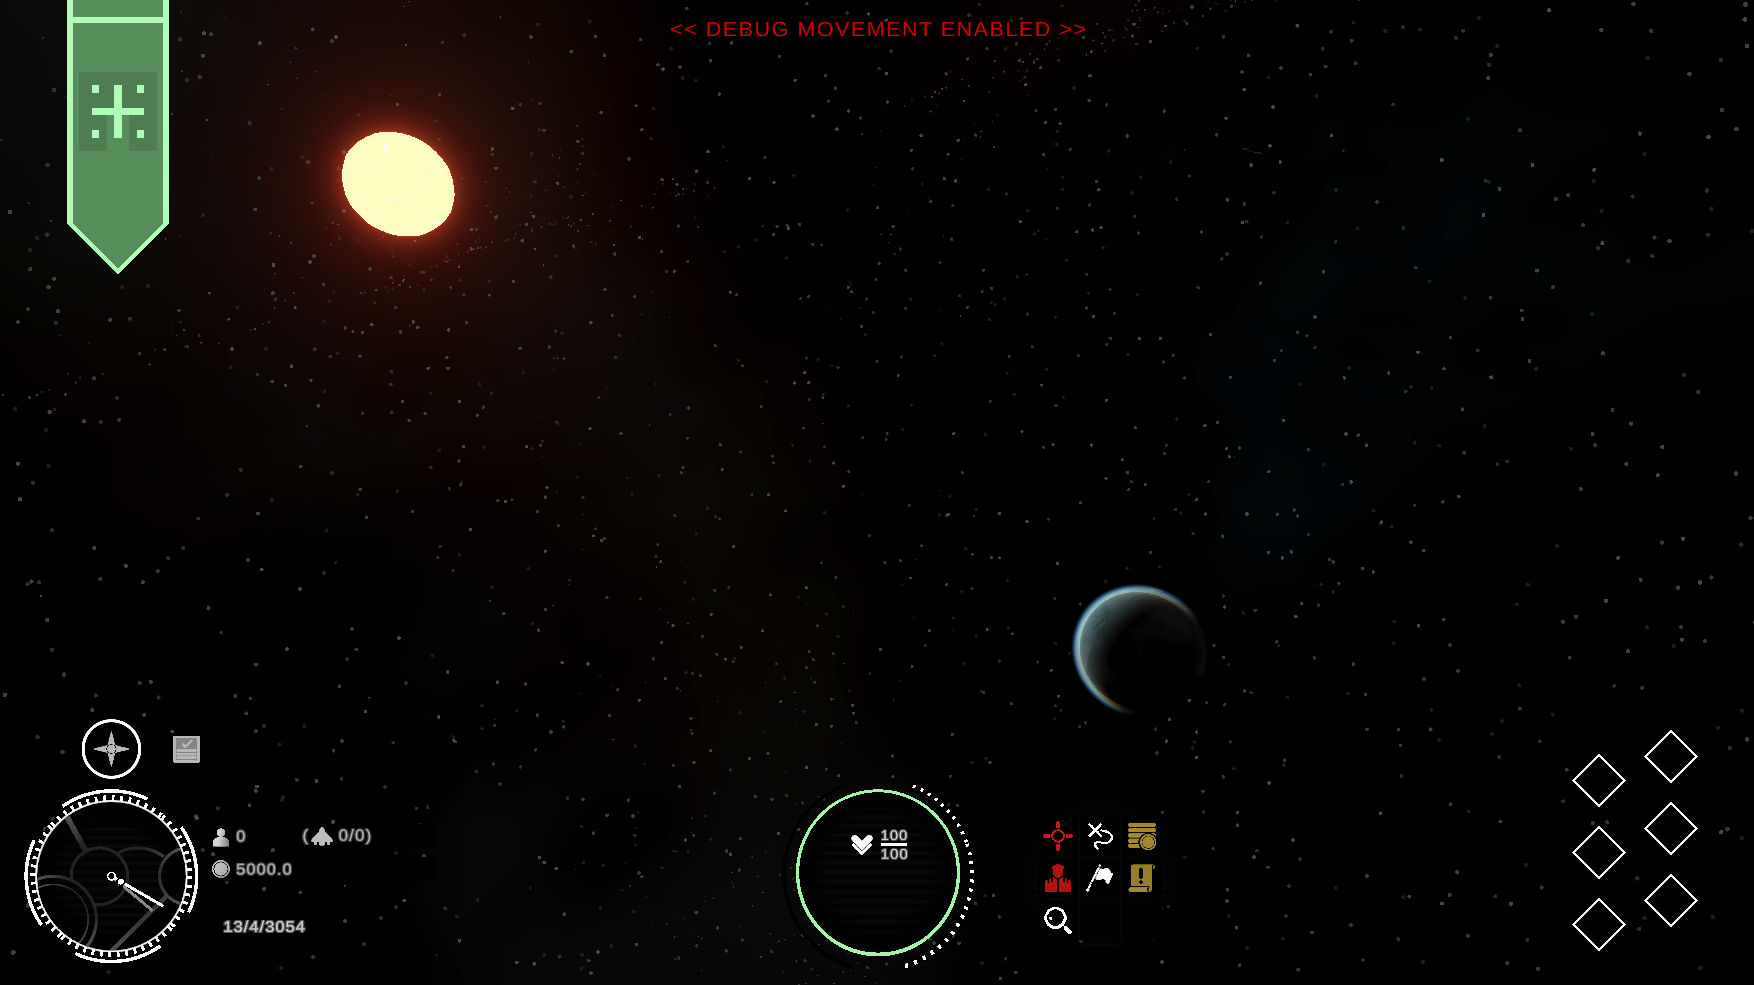
\includegraphics[width=.9\textwidth]{environmentExample1.png}
    \caption{An in-game screenshot of the Sun and a Planet.}
\end{figure}

The Sun shader reuses the planet shader but works with colours pushed into HDR (high dynamic range). A bloom post processing effect is giving the sun it's glow, it utilizes a threshold above typical colour ranges allowing it to singularly affect these types of shaders.

The final place where raymarching is used is in the warp travel effect. Here raymarching's ability to have it's defined shape change over time is used paired with it's ability to define shapes as mathematical equations (in our case a fractal) to create a shifting, otherworldly environment. The blurryness and simplistic colour choice was originally an attempt to limit the performance impact of this particular raymarching shader, however the style worked well for a background element and was maintained through other performance improvements.

\begin{figure}[H]
	\centering
    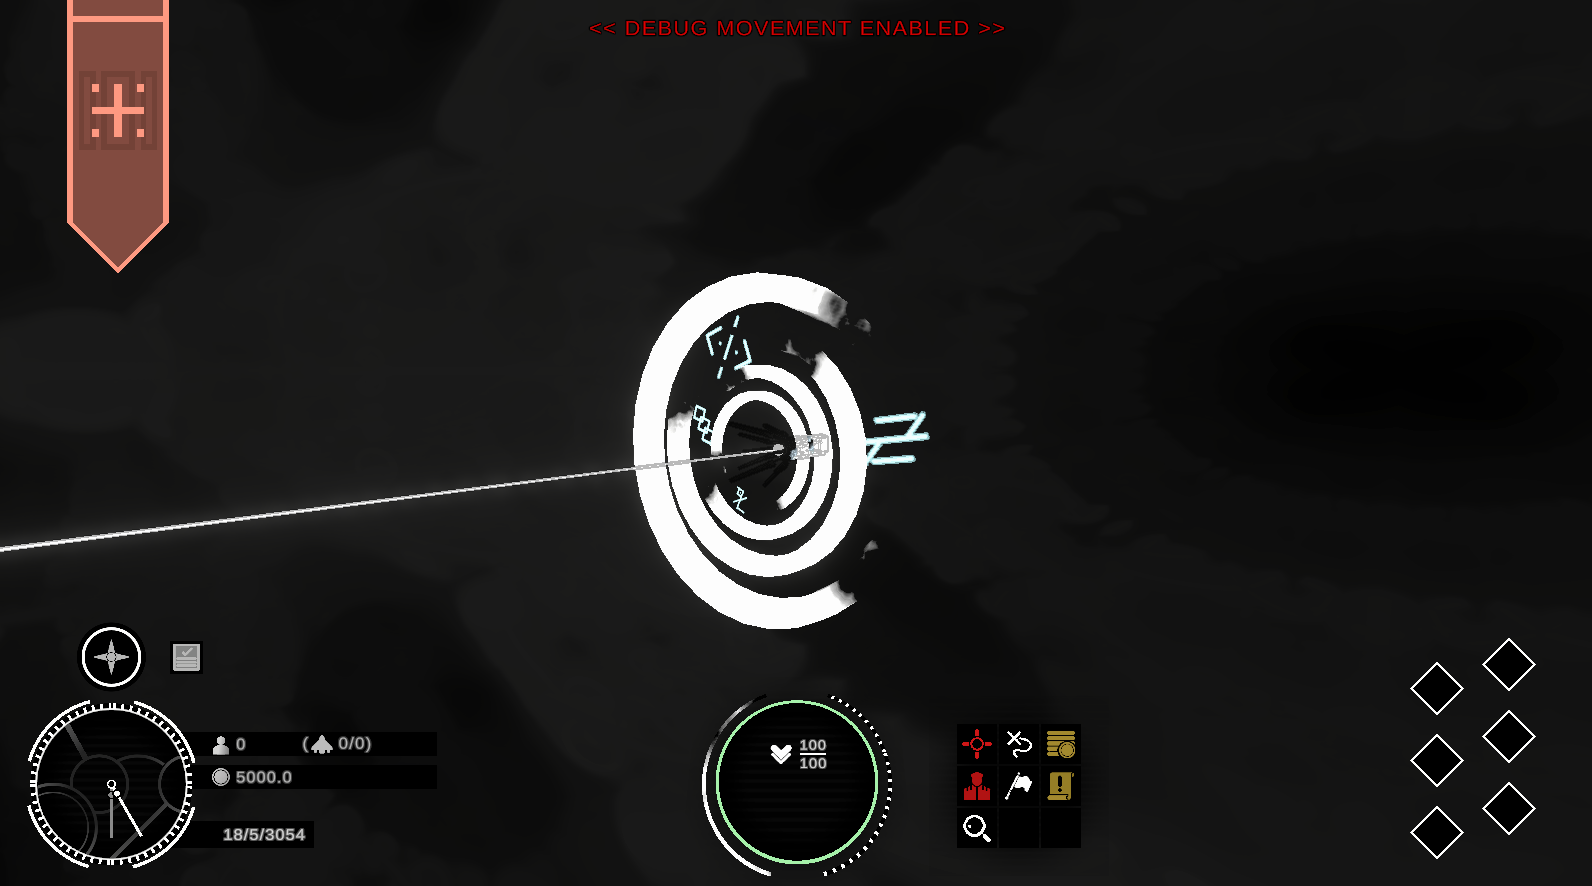
\includegraphics[width=.9\textwidth]{environmentExample2.png}
    \caption{An in-game screenshot of the warp travel effect.}
\end{figure}

The standard 3D models rely heavily on an outline postprocessing effect to accentuate their details, utilizing a simplistic version of hard surface modelling.

\begin{figure}[H]
	\centering
    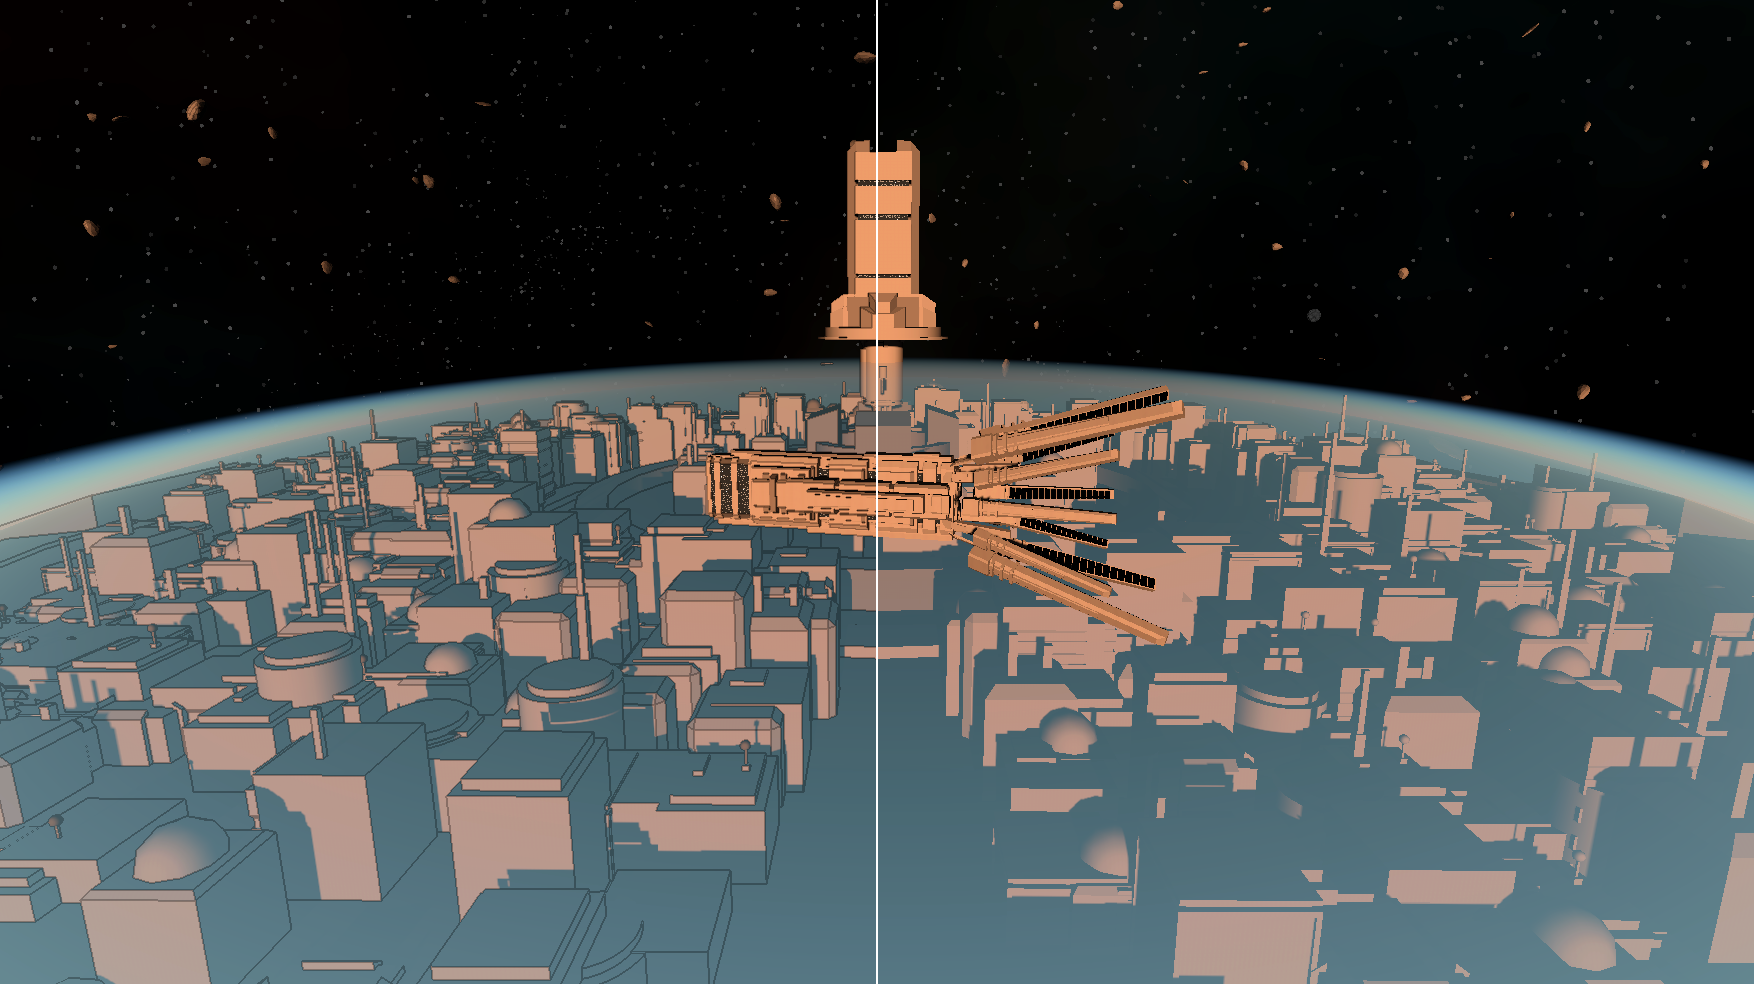
\includegraphics[width=.9\textwidth]{outlineExample.png}
    \caption{An in-game screenshot of a Settlement comparing the game both with and without the outline effect.}
\end{figure}

The blockly models are quick to produce, allowing quick iteration. Above the Settlement is made through several component parts, the buildings, a standard base and the atmosphere shader (borrowed from the planets). To facilitate different layouts, each Settlement generates their buildings when they are first instantiated (based on their underlying data), utilizing the process of instancing to performantly draw many instances of the same meshes.

In the background of the above Figure 5.3, you can see asteroids. These are used as a form of stagnated depth between the environement close to the player and the distant celestial bodies. They act as reference points to help observers undestand the scale of the solar system, without them, faraway elements can seem much closer than they are, which can dramatically hurt the feel of the game.

\subsection{UI}

UI design has gone through more iterations than any other part of the design, UI is one of the primary ways that information is comunicated to the player and so it is vital to get it right. An emphasis has been placed on images over text, however, neccesary textual elements appear on mouse hover. This was done to limit the amount of information presented to the player, in an attempt to limit the upfront complexity of the game. In certain ways this ended up hurting usability and understandability as discussed in the \textbf{User Testing} section below. The UI is composed of singular flat colours, typically black and white, with variations in colour (both gradients and brighter colours) used to apply emphasis (e.g., Interaction Icons, Inventory Item Slots, etc.). It is organized generally into several UI states, with some minor overlap when functionality provided by one state needs to be maintained. 

Several UI elements soley exist to assist players with roleplay, in the "Neutral" (or default) UI state, there are two primary examples of this. First, the player's emblem, customized at the beginning of the run, is displayed in the top left. This is a easy way for the project to showcase a choice made by the player in a constant way. Second, is the clock in the bottom left corner. It is important to the project for the world to feel like it is moving and changing as you play, having a visible clock adds to this by giving a sense of moving time. The clock is also the only animated part of the UI (outside of fade-in transition effects) which helps add additional emphasis to it.

The project also includes a large amount of popups, used for a variety of use cases, including but not limited to, Shop UI, Troop Transfer UI and Action Confirmation UI. These are all set active as default in the Editor when the game is not running, used similarly to a design board. Being able to view all the popups at the same time helps to maintain language and style across the game's UI, including during the creation of new UI States or elements.

\begin{figure}[H]
	\centering
    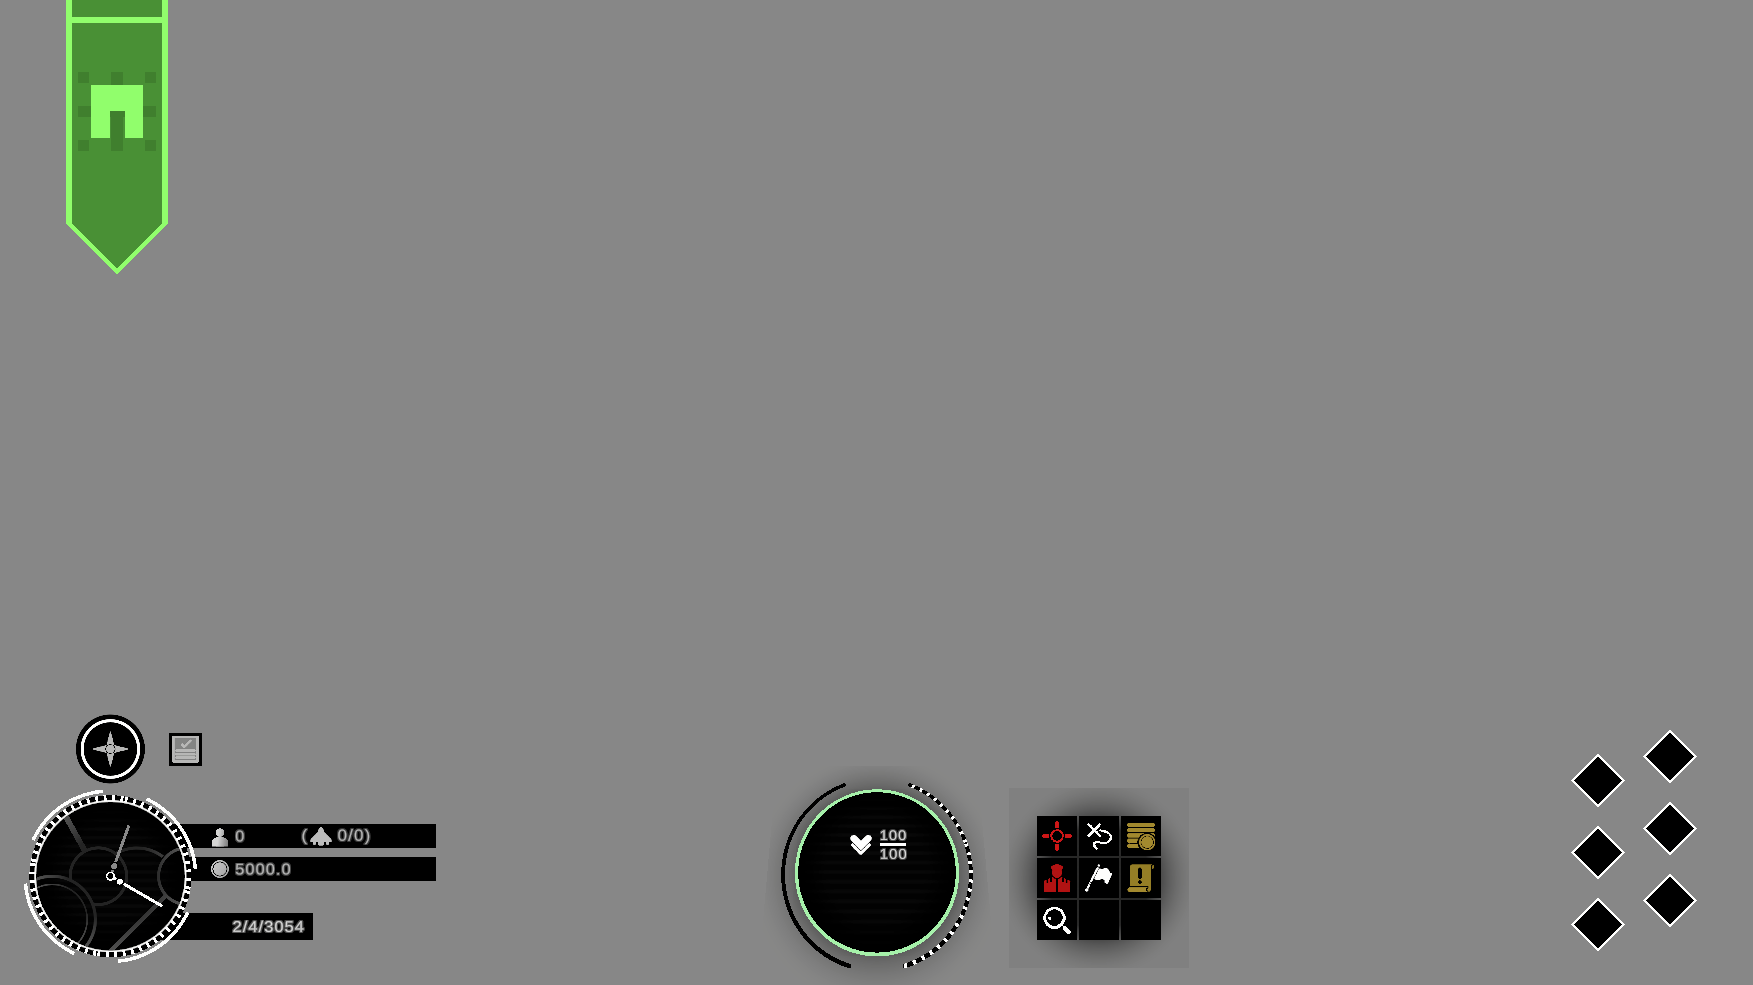
\includegraphics[width=.9\textwidth]{UIExample1.png}
    \caption{The Neutral UI State.}
\end{figure}

\begin{figure}[H]
	\centering
    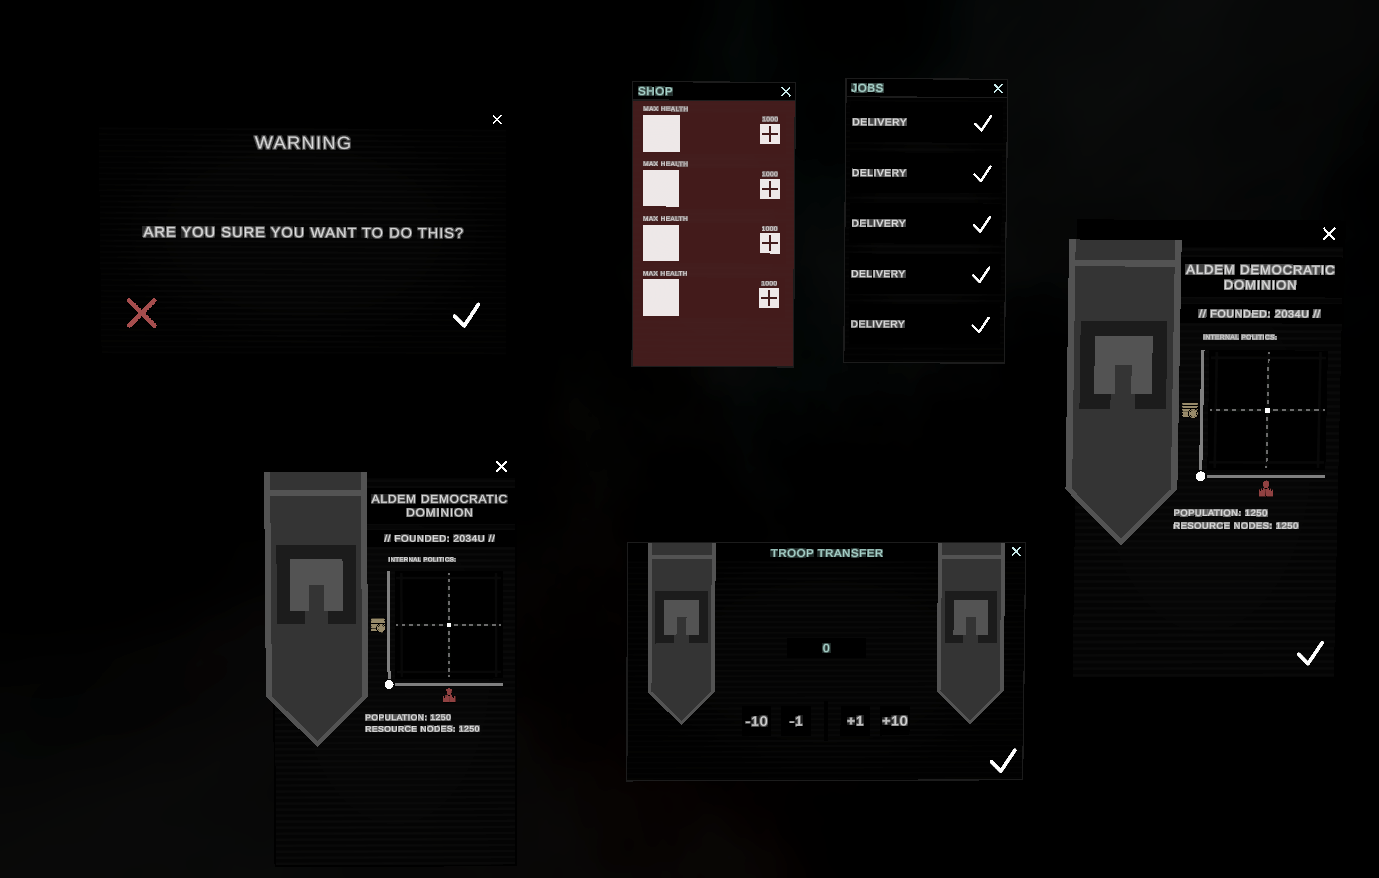
\includegraphics[width=.9\textwidth]{UIExample2.png}
    \caption{Collection of popup windows displayed in Editor.}
\end{figure}

\chapter{Implementation}

The following chapter starts with top down description of the Simulation. This begins with a description of code run by the Simulation (\textbf{Routines}), then it's participants (\textbf{SimObjects} and \textbf{SimEntites}) before finishing with a discussion of the Simulation's backbone (\textbf{SimulationManagement}). Next is a description of how the Simulation is visually displayed, discussing distance and object pooling based drawing techniques. Following that is a discussion of Player Gameplay, including, \textbf{Movement}, \textbf{Interactions}, \textbf{Stats} and \textbf{Items}. The chapter is then finished with a section on UI and the IDisplay interface. 

Due to the complexity of the project (which currently contains 216 scripts), various efforts have been made to simplify the descriptions of the codebase. Focus has been placed on primary structural elements and underlying systems with the exception of the individual \textbf{DataModule} descriptions.

\begin{comment}

Desgin should follow from implementation, as it is a broad overview of the implementation (assuming you actually have some coherence to your code I guess)

Want to have:
	- A list of every data module and explanations of what they do
		- This includes the different levels of interconnectedness of the modules
	(The discussion on modular design should happen in the design section)
	- Discussion of the Simulation Management class and all the things it handles
		- This includes, data lookups, routine running, multithreading, etc.
	- Refactors, notables examples could include the switch from Faction centered code to DataModule centered code and the implementation system iterations


per SimObject implementations could potentially create unexpected behaviour and degenerate gameplay patterns (such as unrepairable relationships)
\end{comment}

\section{Routines}

A \textbf{Routine} is simply code that is run on a Simulation tick. All Routines have a priority value that decides in what order the Routines run, however, certain types of Routines will always run before or after other types. There are four types of Routines:

\begin{enumerate}
        \item Constant Routines

Routines run every single tick, the default type of Routine.

        \item Init Routines

Routines run when data was added last tick and needs to be initialized. Includes a validation check to see if they should act on the new data and always run before any other Eoutines.

        \item Absent Routines

Routines that are only run when specifically invoked. Used typically to test a Routine or temporarily exclude it during testing of other Routines.

        \item Debug Routine

Primary testing Routines. Debug Routines won't be run outside of the Unity Editor or while the Simulation is running history. They are excluded from history ticks as they will typically output some data which will slow down the Simulation considerably. Always run after every other type of Routine.

\end{enumerate}

There are 35 Constant and Init Routines, listed below based on priority.


\begin{table}  [H]
\begin{tabular}{l | l | l }

\hline

\\
\textbf{Init} & \textbf{Constant} \\

PoliticalInit & PlayerSimValuesUpdateRoutine & BattleResolutionRoutine \\ 
TerritoryInit & MilitaryPerTickReset &PoliticalChangeRoutine  \\
TargetableLocationInit & StrategyRoutine & NationDeadRoutine\\
RefineryInit & DesirabilityAttractionRoutine & VoidSwarmDeadRoutine\\
EconomyInit & PopulationSettlementGrowthRoutine & PeriodChangeRoutine \\
EmblemInit & SettlementRoutine & CalamityInitiateRoutine \\
NameInit  & SettlementManagementRoutine & TimerProcessRoutine \\
FeelingsInit & RefineryRoutine & MetaRoutine\\
MilitaryInit & EconomicPowerReductionRoutine & WarEvaluationRoutine\\
& PopulationNaturalChangeRoutine & RandomEventTickRoutine \\
& PopulationBasedTerritoryExpansion \\
& PoliticalEffectsOnFeelingRoutine \\
& MilitaryCapacityFromPopulationRoutine \\
& MilitaryTroopManagementRoutine \\
& WarEffectRoutine \\
& FeelingsMathcingRoutine \\
\\

\hline

\end{tabular}
\end{table}

Most Routines will act directly on \textbf{DataModules} (discussed in 6.3) which allows the Simulation to stay flexible, allowing new Entites with varying behaviours to be added very easily. For example, giving an Entity owned territory in the Game World is as simple as giving it a TerritoryData module and a PopulationData module (with some inital starting population value).

Certain Routines will act directly on \textbf{SimulationEntities}, for example \textbf{NationDeadRoutine} and \textbf{VoidSwarmDeadRoutine}. These are always used as a way to add bespoke behaviour per Entity and in reality all Routines of this type could be refactored to instead act on DataModules. The inital iteration of the Simulation's design acted on Entities by type (at that time only Factions such as Nation and PirateCrew) instead of data. This lead to code patterns involving costly and rigid filtering in each Routine typically to create a list of DataModules to iterate over anyway. These Routines are leftovers from that refactor and have persisted through several other minor design iterations. Ultimately, it is hard to justify spending the time to remove them when the benefits could only be seen when a new Entity is added that would want to share that bespoke behaviour.

\section{SimObject}

Fundamentally all actors in the Simulation are \textbf{SimObjects}, a generic parent class that contains a large amount of virtual methods, following the "Define as Needed" style outlined in Design. All SimObjects are additionally \textbf{DataModules}, allowing them to be stored by \textbf{SimulationEntities} and acted upon by \textbf{Routines} if needed. 

The majority of the code in SimObject is used to interface with non-simulation side systems in a reliable and consistent way, typically with minimal to no extra work per SimObject type. There are five groups of methods, outlined below.

\begin{enumerate}
        \item Draw

Used to define how to visually display any given SimObject, includes methods for inital drawing, cleanup, per-frame updates and post-tick updates.

        \item Battle

Used to define this SimObjects, current health, weapons, on kill reward and on hit reward. Additionally includes a method called when a SimObject is defeated in battle.

        \item Interactions

Helper methods that allow Interactions to check if a SimObject has a Shop or offers Quests. Additionally includes similar methods for the disabled Fuel system.

        \item Reputation

Methods used to adjust the Player's Reputation with an Entity. Reputation as a system should always act on \textbf{FeelingsData} (a \textbf{DataModule}), and hence does not allow a per SimObject implementation. 

	\item IDisplay

A standard implementation of the IDisplay interface, used by UI elements to read (and then display) objects in a consistent way. IDisplay is discussed in detail in a below section.

\end{enumerate}

\subsection{Accessing SimObjects}

While SimObject has many methods that define how it should interact with other systems, those systems need to be able to have some way to access those methods. Primarily this is done through an instance of \textbf{SimObjectBehaviour}, a Unity MonoBehaviour that can interact with Unity's runtime. SimObjects will link themselves to a given behaviour script, typically during their inital draw. The Draw system thus inherently needs to be outside of the scope of SimObjectBehaviour and is handled by \textbf{PlayerLocationManagement} instead.

The only other time SimObjects are handled by neither the Simulation or a SimObjectBehaviour is on the map screen, where \textbf{PlayerMapInteraction} uses the displayed \textbf{TerritoryData} to access the SimObject directly.


\section{SimulationEntity}

Any major participant in the Simulation inheirts from the class \textbf{SimulationEntity} (a child of \textbf{SimObject}). There are currently eight Entites, listed below.

\begin{enumerate}

	\item Player

The Player's Entity, stores any player centric data (e.g., inventory, current stats, current quests, etc.). Most player data was initially stored within an Entity so the current game state could be fully represented using Entites. A few exceptions were taken (e.g., current health, location in world, etc.) for simplicity's sake when it became clear the game state would not need to be saved and loaded in the current iteration.

	\item Nation

The primary Faction the Player interacts with, creates Settlements that give Quests and allow for Trade. Spawns Mineral Deposits and Pirate Crews.

	\item Mineral Deposit

Represents a location in the game's world that has a large resource node.

	\item Pirate Crew

Represents a Pirate Faction, which will raid locations within the game world.

	\item Void Swarm

An example of a Calamity, an Entity that has a large effect on the game world, increasing divergence in generation. Has a chance to spawn at random every ten years.

	\item AntiVoid Knights

An example of a purely reactive Faction. Spawned by Void Swarms a little after their creation and will only target them.

	\item Game World

An implementation of global storage, utilizted in performance critical code where constant data parity ensurance is neccesary but unwieldy to implement. 

	\item Warp

Meant to represent the space during travel. Used primarily to store a Shop that can be accessed by the Player upon buying a particular item.

\end{enumerate}

SimulationEntity includes two primary systems that are used to define the makeup of an entity. These are \textbf{Entity Tags} and \textbf{DataModules}.

\textbf{Tags} are simply Enums, typically used as keys for lookup tables. Entity Tags are general descriptors of an Entity or it's state. They are solely an Enum entry and contain no additional data.  Most types of Entity have a specific type tag to allow for filtering (for example in the execution of the NationDeadRoutine we want to filter for Nations). An example of an Entity State Tag is the "Dead" Tag, which signals to \textbf{Routines} that this Entity needs to be removed or shouldn't be processed.

DataModules are more specific descriptors of Entities, each DataModule is a class, so they can contain arbitrary amounts of data. They are always associated with a Tag (typically an entry in the DataTag Enum) so Routines can filter for them properly. Importantly, DataModules can have multiple layers of inheritance allowing for greater levels of complexity on a per Entity basis.

DataModules vary in their modularity, certain DataModules can function in complete isolation (e.g., EmblemData, NameData, etc.) while others require additional modules to have an sort of functionality (e.g., BattleData, StrategyData, etc.). Consequently DataModule's most important method is \textbf{TryGetLinkedData}, which will attempt to retrieve data (tied to a passed Tag) from the same Entity the target DataModule is from. This allows Routines to functionally work on only DataModules (keeping the Simulation flexible and data-orientated) while having the larger context of the Entity the DataModule is describing.

Certain systems require Entities to communicate but having DataModules tied to a given Entity can make this difficult. Two primary approaches have been taken, splitting data into one sided relationships (that require an Entity and DataModule lookup to get the full picture) and using a form of global storage (\textbf{GameWorld}).

\subsection{Individual DataModules Descriptions}

Below are lists of every DataModule (sorted based on system) and a brief explanation of its use. This should help demonstrate the current scale and complexity of the Simulation.

\subsubsection{Battle System DataModules}

\begin{enumerate}

	\item GlobalBattleData - Global storage for all Battles, used exclusively by \textbf{GameWorld}. An essential part of the \textbf{BattleResolutionRoutine}. All Battles are also \textbf{SimObjects} so they can be drawn. 
 
	\item BattleData - Contains references to the Entity's ongoing Battles. Used primarily to decide where to transfer troops to in the \textbf{MilitaryTroopManagementRoutine}.

	\item MilitaryData - Stores the location of all troops, including ones that don't have a location and are considered in reserve. Additionally dictates what counts as \textbf{Fleet} for this Entity. Used by any Routine relating to \textbf{Battles} or \textbf{TroopManagement}.

	\item RefineryData - Stores data on a \textbf{Ship} building refinery. Used in the \textbf{RefineryRoutine} to produce more troops.

	\item DesirabilityData - Used by \textbf{DesirabilityAttractionRoutine} to pick randomly fights with other Entities at a Location based on a desirability value. Used by \textbf{MineralDeposits}, \textbf{PirateCrews} and \textbf{VoidSwarms} to have other Entities attack them.

	\item StrategyData - Has several virtual functions that are overriden to model various types of strategy. By default \textbf{Ships} are added to \textbf{MilitaryData's} retreat buffer after a battle ends.

	\item RetreatToRservesStrategy - A type of StrategyData that automatically moves all troops back to reserves after a Battle. Used primarily by the \textbf{Player}.

	\item GenocidalStrategy - A type of StrategyData that targets all Entites with Territory. Used by \textbf{VoidSwarms}.

	\item TargetEntityTypeStrategy - A type of StrategyData that targets a specific Entity Type. An entity of that type is chosen and this Entity will continue to attack it until it is destroyed. A new Entity will be then be chosen of the same type (if one exists).

	\item WarStrategyData - A type of StrategyData that stores a list of Entites and then targets them with attacks every tick. This is used by \textbf{Nations} to model campaigns.

	\item ImmediateTargetSpawnSourceData - Forces any \textbf{TargetEntityTypeStrategy} attached to this Entity to target the Entity that spawned it.

\end{enumerate}

\subsubsection{Relationship System DataModules}

\begin{enumerate}
 
	\item FeelingsData - Stores the feelings of one Entity about all other Entites it knows about. Used in many parts of the Simulation to guide action, including choosing to go to war.
	\item ContactPolicyData - Decides whether other Entites inherently know about this Entity and whether this Entity is openly hostile to everyone (e.g., VoidSwarm).
	\item Political Data - Stores the current political climate of an Entity as a value along an Economic and Autority Axis. Affects Entites \textbf{FeelingsData}, a difference in PoliticalData is the most common cause for war between Entities.

\end{enumerate}

\subsubsection{Player Specific DataModules}

These DataModules are used to represent player data. Unlike most other DataModules they are intended to only be used for one Entity.
 
\begin{enumerate}

	\item PlayerInteractions - Stores all the \textbf{Interactions} the Player currently has access too.
	\item PlayerInventory - Stores the currently owned \textbf{Items} and the current amount of currency.
	\item PlayerQuests - Stores the current \textbf{Quests} the Player is on and the max allowed amount of Quests they are allowed to be on.
	\item PlayerStats - Stores the Player's current base stats alongside any extra contributors to those stats (typically provided by Items).

\end{enumerate}

\subsubsection{Other DataModules}

\begin{enumerate}

	\item TerritoryData - Stores all the territories owned by this Entity alongside their border. The border is used in \textbf{PopulationBasedTerritoryExpansion} to add more Territories based on a calcualted upper claim limit. This data is also retrieved to display the map.
	\item SpawnSourceData - Stores information on the Entity this Entity was spawned by. Used by the \textbf{RandomEventTickRoutine} when it spawns a new Entity.
	\item HistoryData - Stores all areas of the world that used to be occupied alongisde information about all the time periods the world has gone through. This is used primarily when the Simulation runs history.
	\item CalamityData - Stores the last tick a Calamity Entity was spawned and the average time between each Calamity. Used soley by the \textbf{CalamityInitiateRoutine}.
	\item EconomyData - Includes a \textbf{Shop} and an estimate of purchasing power. This purchasing power is set based on \textbf{SettlementData} in the \textbf{SettlementManagementRoutine}.
	\item EmblemData - Stores three colours, a main, highlight and shadow alongside a main icon and a backing icon. Used to represent the colours and flag of an Entity. The Player creates an Emblem before running history.
	\item EntitySpawnData - Stores a list of Entity Spawners. Used in the \textbf{RandomEventTickRoutine} to make the world more responsive to particular types of Entities.
	\item NameData - Stores a name for a given Entity. Typically implemented in a bespoke manner for any Entity that needs a name. Used by \textbf{Nations} and \textbf{AntiVoidKnights}.
	\item PoliciesData - Stores all the Policies of a given Entity. This is an incomplete feature but is intended to allow the Player to make long term strategic decisions about their build that they cannot go back on.
	\item PopulationData - Stores a current population count, population cap and natural birth and death rates. Used to help dictate the claim limit in \textbf{TerritoryData} and Settlement cap in \textbf{SettlementsData}.
	\item QuestGiverData - Stores currently pending Quests for the Player to accept. The method used to generate a new quest can be overriden to provide different types based on location.
	\item Settlement - Stores information about a Settlement, this includes storing \textbf{QuestGiverData} and \textbf{RefineryData}. The latter is manually processed in the \textbf{SettlementManagementRoutine} (alongside other Settlement processing) as data lookups only include DataModules that directly belong to \textbf{SimulationEntities}. Like \textbf{Battles}, Settlements are \textbf{SimObjects} so they can be drawn. 

	\item SettlementsData - Stores many Settlements and the max Settlement capacity for this Entity.
	\item TargetableLocationData - Represents a visitable location on the map. Used by many \textbf{Entities} to represent a significant location the Player could travel too.
	\item TargetableLocationDesirabilityData - A child class of DesirabilityData that automatically works for any \textbf{TargetableLocationData}.
	\item TimerData - Stores the tick that this Entity should be destroyed on. Used by \textbf{VoidSwarms} to ensure they don't stay too long and wipe out every Entity continuously.

\end{enumerate}

\section{SimulationManagement}

\textbf{SimulationManagement} is the fundamental backbone of the simulation. It has two primary roles, handling \textbf{DataModule} lookups and running \textbf{Routines} every tick.

SimulationManagement stores several lookup tables that contain references, using an Enum or ID as a key. There are three primary tables, "idToEntity", "tagToEntities" and "tagToData" and one additional table "tagToNewData" (which is cleared after every tick). When an Entity's \textbf{Simulate} method is ran it will first add an entry to "idToEntity" before running the two methods \textbf{InitEntityTags} and \textbf{InitData}. For every new type of Entity those two methods are implemented to define what that Entity is like.
A \textbf{SimulationEntity}'s \textbf{AddData} and \textbf{AddTag} methods will automatically register entries in each lookup table (alongisde adding to a local lookup table in each entity) as needed.

\subsection{Tick Timing and Multithreading}

Simulation ticks are run in two primary modes. First "history" mode, where a number of ticks are batched together onto a seperate thread. This is done on session start to fill the world with established Entities before the player arrives, typical history length is 250 years (108,000 ticks). 
Second is "single tick" mode, where a tick is initiated at the end of our execution of a frame and runs until the start of our execution on the next frame. This means the tick runs while Unity does everything else (e.g., rendering). It is forcefully ended, meaning all execution will stop to let it end if it hasn't already. In "single tick" mode, ticks are started automatically on an interval. Typically this is every three seconds but during travel the interval is shortened to every third of a second.
Additionally ticks can always optionally be made to be instant, meaning they are not executed on another thread. This feature was primarily used for testing and has no use case in the final version of this project.

Running history raises many performance concerns which would otherwise be non-issues, mainly related to the \textbf{BattleProcessRoutine}. Inherently, during time periods where several Nations go to war, many battles take place which results in a large amount of extra processing. Consequently, Battles have been weighted to finish faster. This has to be balanced against the players ability to be involved with Battles as time speeding up during travel can result in Battles ending before the player arrives. The speed up can also not be removed as it causes the rest of the Simulation (during actual gameplay) to slow down considerably, making the world feel static.

\section{Displaying the Simulation Visually}

\textbf{Locations} are a type of SimObject, they act as a wrapper for a \textbf{RealSpacePosition} (Mentioned briefly in the Art Design section above). An RPS works at a higher precision than standard Unity positions, using \textbf{doubles} instead of \textbf{floats}. This is used to combat floating point inaccuracy at the large scales the Simulation works at. \textbf{VisitableLocations} are a child class of Location and act as points of interest for the player.

\subsection{PlayerLocationManagement}

Every frame, \textbf{PlayerLocationManagement} retrieves certain types of DataModules (from SimulationManagement) and uses various lookup tables within them to search for nearby \textbf{VisitableLocations}. The world is divided up into cells with cell centers used as keys for any "spatial" lookup tables. This allows PLM to simply check cells within the players  draw distance rather than iterating over every stored VisitableLocations and doing a manual distance check. Any VisitableLocations found are added to a buffer, and additionally if they are in the buffer left over from the last frame they are removed from it. If they weren't in last frame's buffer than \textbf{InitDraw} is invoked as they have begun being drawn this frame.
At the end of this process any VisitableLocations still in last frame's buffer should no longer be drawn. The \textbf{Cleanup} method is invoked on all these objects before last frame's buffer is cleared and replaced with the buffer created this frame. 

All remaining VisitableLocations will have two update methods called on them \textbf{DrawUpdate} (every frame) and \textbf{DrawUpdatePostTick} (after every Simulation tick).

A typical initial drawing process involves retrieving a model from an object pool (a form of runtime \textbf{GameObject} storage) and placing it in the scene relative to an anchor provided by PLM. The VisitableLocation will link itself to this model's attached SimObjectBehaviour where some additional drawing (based on the data and type of the SOB) might occur. For example, a \textbf{Settlement's} target SOB (of type \textbf{SettlementSimObjectBehaviour}) will generate some instancing buffers to draw all of the neccesary buildings.

Some drawing processes are more complex and require multiple levels of nested drawers, the primary example is \textbf{Battles}. Battles draw process involves creating a sequence of \textbf{ShipCollectionDrawers} which then create \textbf{ShipDrawers}. Each ShipDrawer then gets a model and sets its own position, with some guidance from their parent ShipCollectionDrawer. ShipCollectionDrawers are then drawn or undrawn based on the Simulation state of the Battle rather than distance from the player.
\newline
\newline
Currently the data retrieved by PLM has to be specifically outlined, however the generalized \textbf{TargetableLocationData} (Used by \textbf{MineralDeposits}, \textbf{PirateCrews}, etc.) allows for any flexibility needed. The method used to operate on this data, \textbf{PerformOperationOnNearbyLocations} is reused by \textbf{PlayerMapInteraction}.

\subsection{PlayerMapInteraction}

\textbf{PlayerMapInteraction} draws on top of the normal map UI, using PLM's functionality to find VisitableLocations within the Player's travel range. Each of these locations is given a marker that can be be interacted with by the player. Locations can specify the colour of their marker and whether to include a flashing visual effect via overriding SimObject methods. If any of the Player's Quests include a destination then that is also drawn on the map, in the form of a large beacon.

PMI also handles the drawing of the Interaction Cursor on the map for map enabled \textbf{Interactions}. These include a border highlight mode, a cell selection mode and a line indicator.

\subsection{VisualDatabase}

\textbf{VisualDatabase} is a form of design management, exisiting as a script on a GameObject. It stores both \textbf{Colours} and Icons (Unity \textbf{Sprites}) that can be used by \textbf{SimulationEntites} (in their \textbf{EmblemData}). Some minor hue shift is applied to Colours during the \textbf{EmblemInit} Routine but they will maintain the Saturation and Value. This allows for the creation of a consistent and thought-out style for Entites, while maintaing the randomized nature of the project. A purely random approach would result in an ugly game, harming immersion.

\section{Player Gameplay}

\subsection{Player Movement}

The player's movement is primarily controlled by the script \textbf{PlayerCapitalShip}, the name reflects the original design intention to have the player personally control multiple ships (more akin to Stellaris). Unity's Rigidbody Physics system is used for handiling collisions for the sake of simplicity, however, this system assumes the use of a Unity Transform component as a way to represent movement through the game world. This differs from the higher precision \textbf{RealSpacePosition} system used throughout the rest of the codebase and so the difference between Transform positions across any given frame (assuming the magnitude of the difference is non-zero) needs to be applied to the player's RealSpacePosition. This RPS is reffered to as the \textbf{WorldCenter} (as it is the center from which all RPS based rendering is done, discused above in Art Design), managed by \textbf{WorldManagement}.

Unfortunately, the system as described results in floating point precision errors if the player moves too far away from Unity's world origin. To fix this issue, once the player passes beyond a threshold distance (currently 2000 units) they are seamlessly moved back to the origin. This shift is of course not applied to the WorldCenter RPS, and is typically reffered to as using a "floating origin".

\subsection{Interactions}

All Interactions inheirt from the base class \textbf{Interaction}, similar to \textbf{SimObject} it includes many virtual methods that can be defined as needed. There are two important sets of methods, one for working with \textbf{SimObjectBehaviours} (\textbf{ValidateBehaviour}, \textbf{ProcessBehaviour} and \textbf{GetRange}) and one for working with the map screen (\textbf{ValidateOnMap}, \textbf{ProcessOnMap} and \textbf{GetMapCursorData}), many Interactions will implement both.
The rest of the methods are used for UI definition, including an implementation of IDisplay. Unlike SimObjects there are additional methods for defining draw priority and an icon path (used for automated Sprite Reference caching).

Currently there are eight Interactions, listed below.

\begin{enumerate}

	\item Attack

	Used to toggle targets for the main player ship.

	\item Information
	
	Display's information (Name, Political Leaning) about a given Entity if an SimObject owned by it is targeted.

	\item Shop

	Opens the Shop UI, targeted at the Interaction's target. A Shop can be in Stat Increase mode or Item mode.

	\item Quest

	Opens the Quest accept UI,  targeted at the Interaction's target.

	\item Troop Direct

	Used to direct the Player's military to attack a given place. This place can be a location on the map or a targeted SimObjectBehaviour.

	\item Retreat
	
	Used to retreat the Player's military from a battle they are in.

	\item Travel

	Used to select a Location displayed by \textbf{PlayerMapInteraction} for travel.

	\item Nation Selection

	A special interaction only used at the start of a run. Allows the player to select a starting territory by opening the selection UI. This UI shares functionlity with the Information UI through the use of Unity's prefab system.

\end{enumerate}

An important of an Interaction is defining what things it should be applied to, this is called "validating a target". The static class \textbf{InteractionValidationHelper} includes many helper functions for standard Interaction validations, most validation method implementation are simply calling these functions. 

The player's avaliable Interactions are stored in a \textbf{DataModule} attached to the \textbf{Player} entity. As discussed above, DataModules are intended to fully describe the game state and the player's avaliable Interactions are set up to be malleable. Originally the intention was for certain \textbf{Items} to give the player additional Interactions, for example, a powerful weapon would require a special Interaction, used to direct its use. The item "Divine Battle Logic" is a practical example of this but in the produced vertical slice it has no implemented functionality.

\subsection{Player Stats}

Any given Stat (Attack Power, Move Speed, Max Health, etc.) the player has is composed of two central parts. First, the \textbf{BaseStat} that contains a Stat type identifier and a level. The identifier is used to lookup a List in the "statIdentifierToBaseLevels" dictionary, and the level is used to index into that List, getting a float value that represents the Player's base power in that Stat. Second are the \textbf{StatContributors} which can be of one of three types, \textbf{BaseMultiplier}, \textbf{Addition} and \textbf{FinalMultiplier} (with the default being Addition). StatContributors always hold some value, in the form of a float, but this value is applied differently depending on type. When a Stat is needed the GetStat method is called on the Player's \textbf{PlayerStats DataModule}, within which the target Stat is then calculated before being returned. Stats are calculated using the following equation:

\[((baseStat * productOfBaseMultipliers) + sumOfAdditions) * productOfFinalMultipliers \]

\subsection{Items}

\subsubsection{ItemDatabase}

When the game runtime is initialized, \textbf{ItemDatabase} calls the \textbf{LoadItemsFromFile} method. This takes a file from Resources (a Unity editor to runtime Data Storage solution) called "items" and generates \textbf{Item} objects from it by using a custom interpreter to translate the data. The structure of the "items" data is bespoke but it has similarties to JSON data and it is intended to be edited and understood by humans directly. Below is an example entry for an item that allows the purchase of another item from a special shop alongside modifiying some stats. Text wrapping is not supported, it is used here for readability.

\begin{Verbatim}[frame=single]
### Rare ###
{ item (debug)
	//Buy one item from the special shop
	rarity: "1"
	icon: "specialIcon"
	price: "0.9"
	class: "0"
	moveSpeed: "10"
	attackPower: "0.5 x" 
	attackSpeed: "2 xx"
	name: "Special Shop Token"
	description: "Allows the purchase of one item from the Special Shop, 
will be consumed upon purchase of an item. *item* "
	extra: "Unlike typical Shops, the Special Shop will not 
refresh until it is empty."
	target: "SpecialShopItemBase"
}
\end{Verbatim}

The text between "\#\#\# Rare \#\#\#" starts a new type block. All items until the start of the next type block will use this type, in this case "Rare". The semi colons define a scope, in this case an "item" scope, however, an "alias" scope can be defined as well, allowing for certain words (surounded by the '*' char) to be replaced with predefined text. The text within brackets acts as a flag, allowing decisions to be made about the data before any interpretation begins. Items with the '(debug)' flag, will not be loaded outside of the Unity Editor or if a constant within the ItemDatabase file is set to false.

Within the item scope itself, each line includes a key and a body, seperated by a semi-colon. The key is used to map to a variable inside the new Item object, with the body being interpreted differently based on the variable. Below are descriptors for several of the keys.

\begin{enumerate}

	\item Rarity - Used to define the Rarity level of an Item. Items are stored based on their Rarity so they can be filtered by it.

	\item Icon - Defines an Icon path that a Sprite is loaded from. Relative to "Resources/icons/"

	\item Price - A multiplier to the base item price, currently 1000. This relative style approach helps with balancing.

	\item Class - Defines the class of an item as an index into an enum. Class is used purely for flavour and has no gameplay impact.

	\item Name, Description and Extra - Used in implementations of IDisplay functions so Items can be displayed on UI elements.

\end{enumerate}

If no direct mapping is found then the line is treated as a Stat line, where the key is assumed to correspond to a Stat identifier (if no corresponding Stat exists then that data is just stored and never used for anything). Within the body of the Stat line, the number of 'x' characters define it's type, 0 for \textbf{Addition}, 1 for \textbf{BaseMultiplier} and 2 for \textbf{FinalMultiplier}.

\subsubsection{ItemBase}

\textbf{ItemBase} is a wrapper class for an Item, it includes several important helper functions alongside tracking the \textbf{StatContributors} of a given Item so they can be easily removed. ItemBases are generated with the help of \textbf{ItemHelper's} \textbf{Wrap} method, taking in a target Item to wrap. Typically the returned object will simply be of type ItemBase, however, within an Item's source data a "target" can be specified. ItemHelper will use this to return an instance of a child type instead allowing for flexible Item implementations. In the above case, code will check if the Player's Inventory contains an item of type \textbf{SpecialShopItemBase} before allowing them to open the special shop.

\begin{comment}

Need to talk about loading sprite images
Loading in items (structure of the items file) and storing them
ItemBase as a wrapper
Applying stat changes
Descriptions as an implementation of IDisplay
Custom ItemBase wrappers

\end{comment}

\section{UI}

All UI in the game is built on top of the \textbf{UIManagment} class, which controls the current \textbf{UIState}. Typically you can only transition to a new \textbf{UIState} (referred to as activating a state) from the Neutral state, this model helps segment the UI into specific parts. Additionally it allows the control of UI to be simplified, into Neutral and non-Neutral, which is useful for limiting certain actions when UI is active. In reality, certain UI States require Neutral UI to be active alongside them (for example, the Map), referred to as \textbf{co-enabling Neutral}, as such \textbf{pure Neutral} has it's own set of checks for other systems to use. Very rarely, one non-neutral UIState needs to transition directly to another non-neutral UIState, within the vertical slice this is done only when transitioning from History UI to Nation Selection UI. This behaviour has to be specifically enabled otherwise the method used to change UIState does nothing.

\subsection{IDisplay}

\textbf{IDisplay} is an interface that can be passed to many UI element classes. Those classes will then call IDisplay's methods to help draw their displays, for example \textbf{SlotUI}. IDisplay has four methods, listed below alongside a description.

\begin{enumerate}

	\item GetTitle

Returns a String. Used to set the text of headers, typically returns the name of the interface implementer.

	\item GetDescription

Returns a String. Used as additional text that describes the interface implementer.

	\item GetExtraInformation

Returns a String. Typically used for information that is considered mostly unnecessary or only necessary once. For example, it is used to display the uses of Stats (e.g., Move Speed, Max Health, etc.) given by an \textbf{Item}.

	\item GetIcon

Returns a Sprite. Used by non-text based UI Elements, for example, the image used in \textbf{SlotUI}. Typically returns a cached Sprite loaded from \textbf{Resources}, alternatively returns \textbf{null}, which is interpreted as a white square by Unity (this is a simplification of how Unity's UI shaders work).

\end{enumerate}

Everything from \textbf{Items} to \textbf{Locations} implements IDisplay. Having an interface for UI element drawing allows UI elements to be easily generalized and reused, alongside having multiple different types of UI elements use the same single source data. For example, different slots can draw themselves using IDisplay and then also pass that data to \textbf{DisplayOnHover} (a class that handles almost all mouse over events). 

\chapter{Testing And User Evaluation}

\section{Debug Tools}

During the course of this project, various debug tools have been used to assist with development. First is MonitorBreak's console, in particular the \textbf{ConsoleCMD} attribute which is used to execute arbitrary code at runtime. This allows for the spawning of specific Entities, easy acquisition of specific Items, printing readouts of Entity data to console and removal of animations (for the sake of testing speed) alongside many other use cases. Second are the Debug and Absent Routines (discussed in Implementation above), unlike other forms of testing these are typically temporary (used to test a single Simulation system) and are not included in the final version of the game. Unity's Debug class was also used generously, typically to draw debug lines or as a form of quick and dirty logging.

Alongside specific tools, typical programming testing features (such as Asssertions) are used throughout the code base. For example, in the \textbf{ItemHelper} class's \textbf{Wrap} method, it is asserted that the \textbf{Item} being wrapped is not \textbf{null} as there is no way for the code to attempt to wrap a null object if the \textbf{ItemDatabase} is functioning as expected.



\section{User Testing and Usability}

The primary goal of testing in this project was to gauage the game's usability, this is for two reasons. First, the vertical slice of the game accurately demonstrates what the game could look like but falls short of being a fully playable experience, this makes gameplay testing much less useful. Second, even in an unfinished state, the gameplay loop has a large amount of upfront complexity, it is important that players are able to get started with the game in the first place.

Several features have been implemented in response to player feedback, particularly in respect to Interactions. When mousing over a target all possible interactions are now shown, with the currently selected interaction being highlighted. All Interaction selection buttons now also use \textbf{DisplayOnHover} to show their names to the player on mouse over, this was in response to specific feedback that the icons were unclear. Additionally when using certain Interactions (e.g., Attack), a prompt is now displayed asking if you are sure about what you are doing. This is included to prevent players from misclicking and attacking one of their allies, typically resulting in being attacked by that ally and lowering the player's reputation with them.

\chapter{Conclusion}

\renewcommand\bibname{References}
\begin{thebibliography}{9}
\bibitem{stellarisBeginner}
Stellaris Community, "Beginner's guide", "Stellaris WIki", 21 October 2024, \href{https://stellaris.paradoxwikis.com/Beginner\%27s_guide}{https://stellaris.paradoxwikis.com/Beginner\%27s\_guide}
\bibitem{stellarisBattleDecision}
Stellaris Community, "Crisis/Endgame crisis factions/Extradimensional Invaders/Successfully repelling the Extradimensional Invaders", "Stellaris Wiki", 18 October 2024, \href{https://stellaris.paradoxwikis.com/Crisis#Successfully_repelling_the_Extradimensional_Invaders, Crisis Solution Link}{https://stellaris.paradoxwikis.com/Crisis}
\bibitem{rtsUncertainty}
Jónsson, B. Pages 6 to 7, "REPRESENTING UNCERTAINTY IN RTS GAMES"
\bibitem{stellarisPerformanceReview1}
"Skullcrusher", "Stellaris Steam Review", "Steam", 11 September 2022, \href{https://steamcommunity.com/profiles/76561198026459371/recommended/281990, "Review Link"}{https://steamcommunity.com/profiles/76561198026459371/recommended/281990}
\bibitem{stellarisPerformanceReview2}
"A Random Fish", "Stellaris Steam Review", "Steam", 18 October 2019, \href{https://steamcommunity.com/id/ARandomFish/recommended/281990, "Review Link"}{https://steamcommunity.com/id/ARandomFish/recommended/281990}
\bibitem{additionsLicense}
"MonitorBreak", "License", "Github", 14 November 2022, \href{https://github.com/Monitor-Break/Additions/blob/main/LICENSE}{https://github.com/Monitor-Break/Additions/blob/main/LICENSE}
\bibitem{unity}
"Unity Technologies", "Home Page", "Unity Website", \href{https://unity.com/}{https://unity.com/}
\bibitem{unreal}
"Epic Games", "Home Page", "Unreal Engine Website", \href{https://www.unrealengine.com/en-US}{https://www.unrealengine.com/en-US}
\bibitem{godot}
"Godot Foundation", "Home Page", "Godot Website", \href{https://godotengine.org/}{https://godotengine.org/}
\bibitem{bcs}
"British Computer Society", "Code of Conduct", "BCS Website", \href{https://www.bcs.org/membership-and-registrations/become-a-member/bcs-code-of-conduct/}{https://www.bcs.org/membership-and-registrations/become-a-member/bcs-code-of-conduct/}
\bibitem{stellaris}
\textit{Stellaris} (2016), PC [Game], Paradox Interactive
\bibitem{crusaderkings}
\textit{Crusader Kings} (2004), PC [Game], Paradox Interactive
\bibitem{discoelysium}
\textit{Disco Elysium} (2019), PC [Game], ZA/UM
\bibitem{steam}
Valve, "Steam Homepage", "Steam", 04/11/2024, \href{https://store.steampowered.com/}{https://store.steampowered.com/}
\end{thebibliography}

\begin{appendices}
\chapter{Project Proposal}
\noindent\makebox[\linewidth]{\rule{\paperwidth}{0.4pt}}
\begin{center}
\textbf{Space Based Simulation and Tactics Game}
\end{center}

\textit{Candidate Number: 267533}

\textit{Supervisor Name: Dr Paul Newbury}

\textbf{Aims}
\newline
Many games try to create a branching narrative. When done well this can imbue even non impactful decisions with a sense of weight, this feeling that everything contributes. On the other end, when done poorly, all decisions can become meaningless, whether they are impactful or not. What matters is the player thinking they’re having an impact.

In this project I intend to (with the constraints inherently imposed by solo indie development in mind) create a video game that creates an emergent narrative through gameplay rather than text, maximising the feeling of impact for the player. This form of narrative is seen commonly in the large-scale real-time strategy genre (e.g. Stellaris, Crusader Kings, etc.) where interlocking systems tell the stories of large factions. There will be some simplification to allow users that would normally be turned off by the upfront complexity of these games to also engage with the final product.

\textbf{Objectives}

\underline{\textit{Primary Objectives}}

\begin{enumerate}
	\item Research existing games in the genre, identifying their gameplay focus points \& style.
	\item Examine what games in the genre do well and what they do poorly.
	\item Conduct interviews with 5+ potential players, utilizing insights gained in Primary Objectives 1 and 2 to shape the questions asked
	\item Examine what games in the genre do well and what they do poorly.
	\item Use information from all Previous completed Objectives to design a game that tells player driven stories.
	\item Create a beta version of the completed game that can be tested and critically evaluated, both by me and potential players.
	\item Use insights gained from Primary Objective 5 to iterate and improve on the beta version.
	\item Ultimately finish a vertical slice that would lack some features but showcase accurately what the final product could look like.
\end{enumerate}

\underline{\textit{Extension Objectives}}

\begin{enumerate}
	\item Perform Primary Objectives 5 and 6 continuously to further improve the final product.
	\item Conduct critical evaluation using the vertical slice, in the same manner as Primary Objective 5.
	\item Utilize the insights gained in Extension Objective 2 to further improve upon the vertical slice, expanding it into a fully completed game.
	\item Implement additional simulated features into the game, refining the model.
	\item Implement online leaderboard functionality for various statistics.
	\item Release the fully completed game on platforms such as Steam and Itch.io.
\end{enumerate}

\textbf{Relevance}

This project reflects my intended career path, as someone that has already been working with Unity and C\# for the last five years. During my gap year (2021 - 2022) I went through the full development process, releasing a 2D game on Steam in early July. Since then, I’ve been working on both my development and 3D skills and hope to release another game I’ve been working on a couple months post university.

By doing this project I hope to further both my coding and artistic skills, combing them to create a hopefully great video game. This project tests both of those disciplines alongside my ability to gather effective feedback and implement proper HCI principles.

\textbf{Resources Required}

I will require use of study rooms/seminars to conduct in person user testing. Testing will also be conducted online but that should require minimal resources. No funding will be required as I expect to purchase games used for market research myself. I also expect to pay for the Steam direct fee if Extension Objective 6 is completed.

Some use of lab computers is required (primarily on Mondays) though I intend to use my home PC on a day-to-day basis. This is due to several factors; my extensive backlog of previous projects I can pull reusable systems/assets from, the comfortability of the workspace and the ease of access, alongside various others.

\textbf{Time Management}

\begin{table}[htbp]
\begin{tabular}{|c|c|c|c|c|c|c|c|}
\hline
 & Monday & Tuesday & Wednesday & Thrusday & Friday & Saturday & Sunday \\
\hline
9:00 &&&&&&& \\
\hline
10:00 & Lecture & & Lecture &&&& \\
\hline
11:00 & \textbf{Project} &&&&&  \textbf{Project} &  \textbf{Project} \\
\hline
12:00 & \textbf{Project} & & \textbf{Project} & \textit{Seminar} & \textbf{Project} & \textbf{Project} & \textbf{Project} \\
\hline
13:00 & Lab & Lecture &  \textbf{Project} & &  \textbf{Project} &  \textbf{Project} &  \textbf{Project} \\
\hline
14:00 &&&&&&& \\
\hline
15:00 & Lecture & & & Lab & Lecture && \\
\hline
16:00 & Lecture & & & Lab & Lecture && \\
\hline
\end{tabular}
\label{tab:schedule}
\end{table}

Project time per week is equal to 12 hours. This acts as a minimum goal and (due to my general passion for the subject matter) I will likely do more depending on the week. Any blank slots will be used for other modules, whether coursework or study. The minimum time spent each week will increase depending on unseen factors such as unintended scope creep or hidden complexity.

I intend to have the initial early beta version of the finished shortly after the interim report (Week 8 to 9 of Term 1), utilizing feedback gained over the Christmas break. I then expect to finish the final vertical slice a couple weeks before the final report is due. Any additional time gained, by being ahead of schedule, will be used to complete extension objectives, primarily Extension Objectives 1 and 2.

\noindent\makebox[\linewidth]{\rule{\paperwidth}{0.4pt}}

\begin{center}
\textbf{This proposal has been adapted from Word to \LaTeX{}, so exact formatting differs from the original proposal document. Structure and content remains the same.}
\end{center}

\chapter{Signed Ethical Compliance Form}

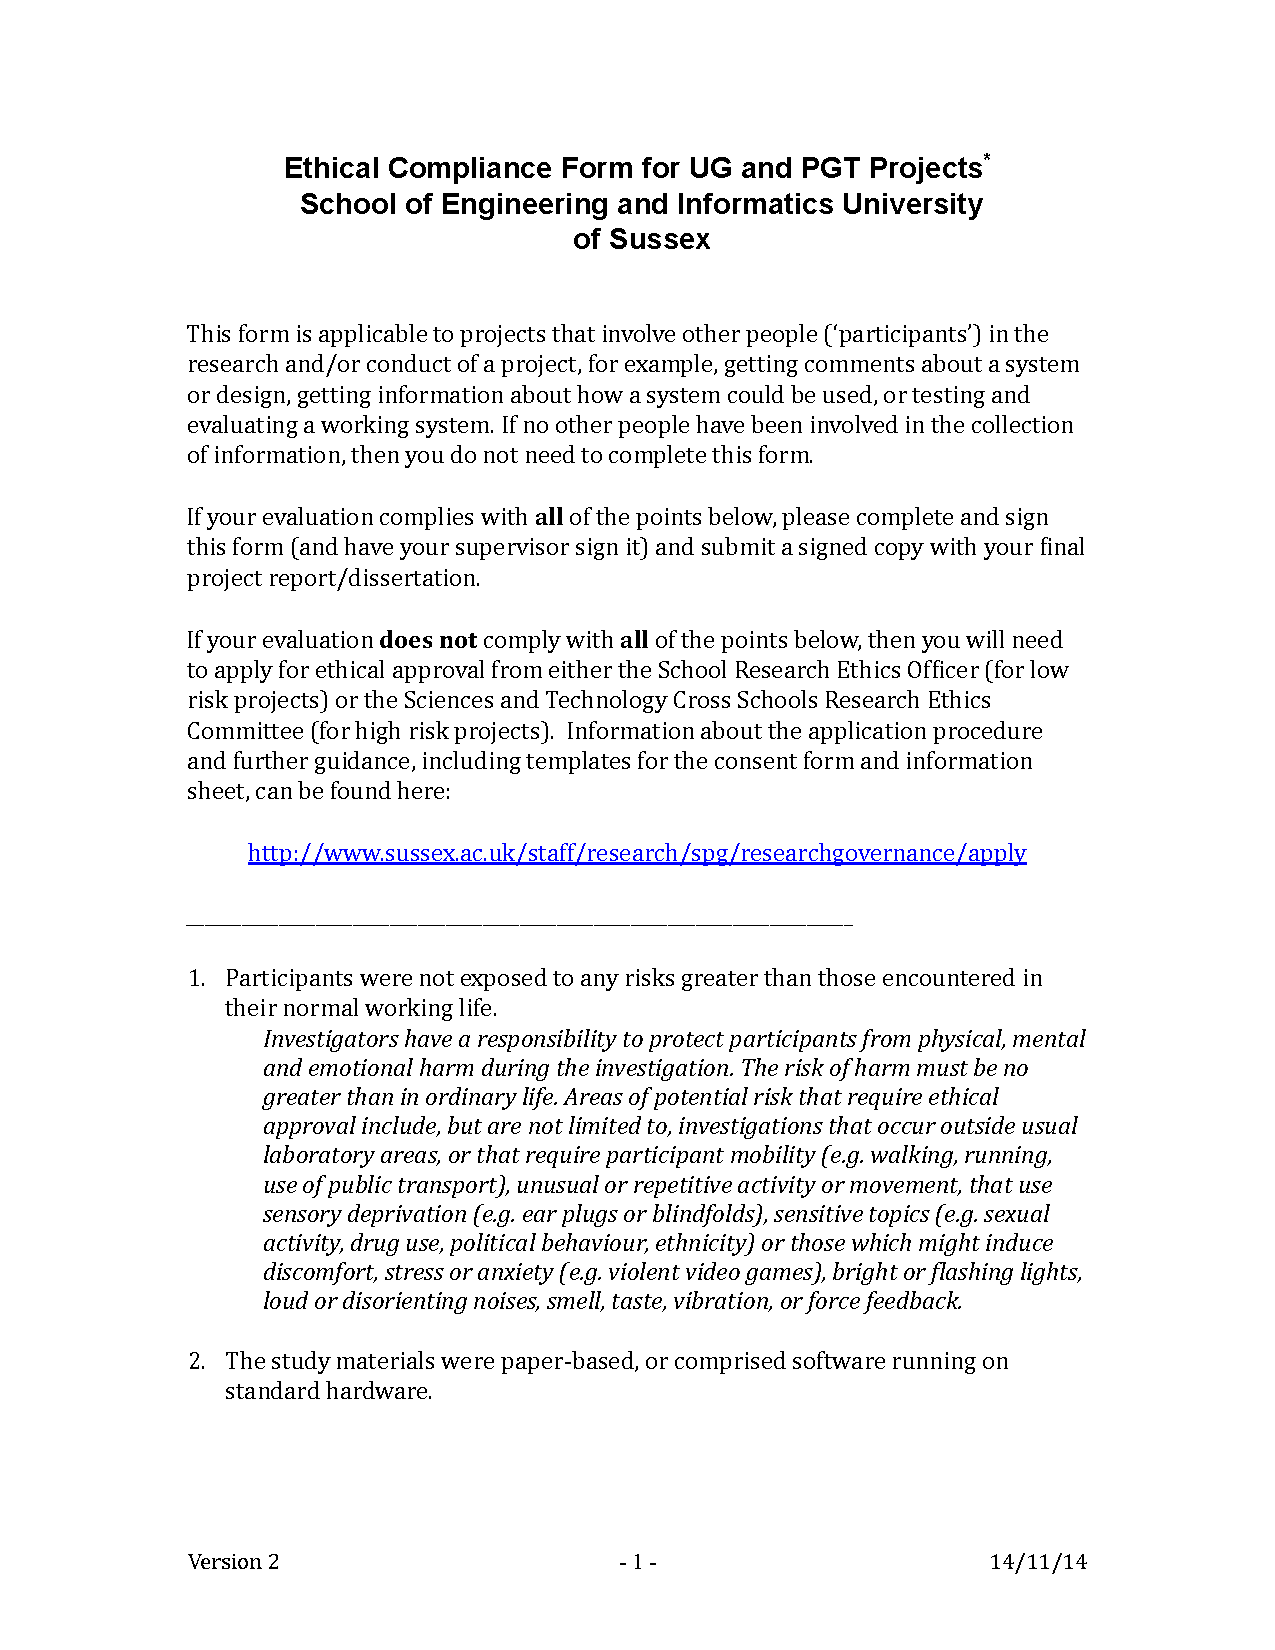
\includepdf[pages=-]{AlexanderNolesEthicalComplianceForm.pdf}

\end{appendices}
\end{document}